\documentclass{article}
%\usepackage{style}
\usepackage[ruled, algo2e]{algorithm2e}
\usepackage{amsmath, amsfonts, amsthm}

%\usepackage{graphicx, epstopdf}
\usepackage{color}
\usepackage{cite}
\usepackage{indentfirst}
\usepackage{geometry, graphicx}
\usepackage[title]{appendix}
\usepackage{algorithm, algorithmic}
\usepackage{bm}
\usepackage[hidelinks]{hyperref}
\usepackage{multirow}
\usepackage[tight]{subfigure}
%\usepackage{ulem}
\geometry{left = 5em, right = 5em}
\usepackage{listings}
\usepackage{xcolor}
\usepackage{subfigure} 
%% notation macro
\newcommand{\OB}{\Ocal\B}
\newcommand{\Rt}{\operatorname{Rt}}
\newcommand{\Grad}{\operatorname{grad}}
\newcommand{\sign}{\operatorname{sign}}
\newcommand{\diag}{\operatorname{diag}}
\newcommand{\tfo}{\textbf{1}}
\newcommand{\E}{\mathcal E}
\newcommand{\F}{\mathcal F}
\newcommand{\T}{\mathcal T}
\newcommand{\I}{\mathcal I}
\newcommand{\Ocal}{\mathcal O}
\newcommand{\Ibf}{\mathbf I}
\newcommand{\Y}{\mathcal Y}
\newcommand{\Ybf}{\mathbf Y}
% \newcommand{\U}{\mathcal U}
\newcommand{\R}{\mathbb R}
\renewcommand{\P}{\mathcal P}
\newcommand{\uP}{ \mathcal \uline P}
\newcommand{\V}{\mathcal V}
\newcommand{\A}{\mathcal A}
\newcommand{\B}{\mathcal B}
\newcommand{\G}{\mathcal G}
\newcommand{\Hcal}{\mathcal Hcal}
%\newcommand{\R}{\mathbb R^2}
\newcommand{\Z}{\mathbb Z}
\newcommand{\Eb}{\mathbb E}
% \newcommand{\C}{\mathbb C}
\newcommand{\laplacian}{\triangle}
\newcommand{\grad}{\nabla}
\renewcommand{\div}{\textrm{div~}}
% cf
\newcommand{\iprod}[2]{\left\langle #1, #2 \right\rangle}
\newcommand{\II}[1]{\mathbb{1}\left\{#1\right\}}
\newcommand{\nrm}[1]{\left\|#1\right\|}
\newcommand{\bH}{\mathbf{H}}
\newcommand{\eps}{\varepsilon}
\newcommand{\DD}{\mathbb{D}}
\newcommand{\RR}{\mathbb{R}}
\newcommand{\cO}{\mathcal{O}}
\newcommand{\cB}{\mathcal{B}}
\newcommand{\PP}{\mathbb{P}}
\newcommand{\EE}{\mathbb{E}}
\newcommand{\relu}{\operatorname{ReLU}}
\renewcommand{\II}[1]{\mathbb{I}\left\{#1\right\}\}}

\newcommand{\diff}[2]{\frac{\partial #1}{\partial #2}}
\newcommand{\difff}[3]{\frac{\parial #1^2}{\partial #2 \partial #3}}
\newcommand{\diFF}[2]{\frac{\partial #1^2}{\partial^2 #2}}
\newcommand{\diam}{\text{ diam }}
%% non-noation macro
\newcommand{\IN}{\text{  in  }}
\newcommand{\ON}{\text{  on  }}
\newcommand{\st}{\text{s.t.  }}
\newcommand{\tbc}{{\color{red}[TBC]}}
\newcommand\ldq\textquotedblleft
\newcommand\rdq\textquotedblright{}
\newcommand\mb\mathbb
\newcommand\mf\mathbf
\newcommand\tf\textbf
\newcommand{\revise}[1]{{\color{blue}#1}}

\newcommand{\return}{\textbf{return~}}
\DeclareMathOperator{\argmin}{arg~min}
\DeclareMathOperator{\argmax}{arg~max}
%% enviorment
\newtheorem{proposition}{Proposition}
\newtheorem{definition}{Definition}
\newtheorem{corollary}{Corollary}
\newtheorem{remark}{Remark}
\newtheorem{assumption}{Assumption}
\newtheorem{Proposition}{Proposition}
\newtheorem{Definition}{Definition}
\newtheorem{Corollary}{Corollary}
\newtheorem{Remark}{Remark}
\newtheorem{Assumption}{Assumption}
\newtheorem{Condition}{Condition}
\newtheorem{condition}{Condition}
\newtheorem{theorem}{Theorem}
\newtheorem{lemma}{Lemma}
\setlength{\parindent}{1.5em}
\definecolor{mygreen}{rgb}{0,0.6,0}
\definecolor{mygray}{rgb}{0.5,0.5,0.5}
\definecolor{mymauve}{rgb}{0.58,0,0.82}
\lstset{ %
	backgroundcolor=\color{white},      % choose the background color
	basicstyle=\footnotesize\ttfamily,  % size of fonts used for the code
	columns=fullflexible,
	tabsize=4,
	breaklines=true,               % automatic line breaking only at whitespace
	captionpos=b,                  % sets the caption-position to bottom
	commentstyle=\color{green},  % comment style
	escapeinside={\%*}{*)},        % if you want to add LaTeX within your code
	keywordstyle=\color{blue},     % keyword style
	stringstyle=\color{mymauve}\ttfamily,  % string literal style
	frame=single,
	rulesepcolor=\color{red!20!green!20!blue!20},
	% identifierstyle=\color{red},
	language=matlab,
	numbers=left,
}
\title{\textbf{\showtitle}}
\author{\showauthor}
\usepackage{indentfirst}
\usepackage{fancyhdr}  
\pagestyle{fancy}

\renewcommand{\algorithmicrequire}{\textbf{Input}}
\renewcommand{\algorithmicensure}{\textbf{Output}}
%\lhead{\textbf {\showtopic} }
%\chead{} 
%\rhead{\textbf {\showabs} }
%\lfoot{} 
%\cfoot{\thepage}
%\rfoot{} 
%\renewcommand{\headrulewidth}{0.4pt} 
%\usepackage{lineno}
%\linenumbers
\usepackage{caption}

\newcommand{\be}{\begin{equation}}
\newcommand{\ee}{\end{equation}}
\newcommand{\mL}{\mathcal L}
\newcommand{\dA}{\Delta(\A)}
\newcommand{\dB}{\Delta(\B)}
\newcommand{\KL}{\mathrm{KL}}
\newcommand{\dualgap}{\Operatorname{DualGap}}
\newcommand{\prox}{\mathrm{prox}}
\newcommand{\proj}{\mathrm{proj}}
\title{Variants of Stochastic Gradients Algorithms}
\date{\today}	
\author{Ruicheng Ao 1900012179}
\begin{document}
\maketitle
\section{Problem description}
In this homework, we focus on the unconstrained optimization algorithm in which the objective function can be de formulated into the form
\begin{equation}\label{prob}
\begin{array}{cc}
\min &L_\lambda(x,y)=\frac{1}{n}\sum_{i=1}^n f_i^(w)+\lambda\|w\|_2^2,
\end{array}
\end{equation}
% where $f_i(w) = \log (1+\exp(-y^iw^\top x^i))$ and $\lambda > 0$. With a simple computation one can get
wherer $f_i(w) = 1-tanh(y^iw^\top x^i)$ and $\lambda >0$. With a simple computation we get
\begin{equation}\label{grad}
	\nabla_w f_i(w) = -1+y^ix^i\tanh(y^iw^\top x^i)^2.
\end{equation}
% \begin{equation}\label{grad}
% \nabla_w f_i(w) =\frac{\exp(-y^iw^\top x^i)}{1+\exp(-y^i z^\top x^i)}(-y^ix^i).
% \end{equation}
The gradient $\nabla L_\lambda $ involves the sum of $n$ different terms, which makes the computation costly. As a result, several stochastic methods using the technique of sampling are widely used \cite[Section 8]{goodfellow2016deep}. In our experiments, we mainly focus on four of the first-order algorithms : Adagrad, Adam, SGD with momentum \& linesearch, RMSprop and show their efficiency. The first two are required and SGD with momentum \& linesearch, RMSprop are as extra credit.
\section{Algorithm description}
In this section, we introduce Adagrad, Adam, SGD with momentum, SGD with line search and RMSprop, and give the general frameworks.
\subsection{Adagrad}
Adagrad is one of the most famous algorithms in deep learning, named by adaptive gradient algorithm. It considers adding an accumulated second-order moment of gradient in order to accelerate the convergence. This scheme can adaptively adjust the gradient without fine tuning, which enjoys good performance on many problems \cite{goodfellow2016deep}. The framework of Adagrad is given in Algorithm \ref{adagrad}.
\begin{algorithm}[H]
	\caption{Adagrad}
	\begin{algorithmic}[1]\label{adagrad}
		\REQUIRE{Learning rate $lr$, regularization parameter $\delta$, batch size $bs$}
		\STATE{Set $k=0$}
		\STATE{Set $r=\vec 0$}
		\WHILE{Do not converge}
		\STATE{Sample a minibatch set B of size $bs$ from the training set}
		\STATE{Compute sampled gradient $g^k = \frac{1}{bs}\nabla_w\sum_{i\in B}f_i(w)+2\lambda w$}
		\STATE{Update $r=r+g^k\odot g^k$}
		\STATE{Update $w^{k+1} = w^k-\frac{lr}{\sqrt{\delta+r}}*g^k$}
		\STATE{$k=k+1$}
		\ENDWHILE 
	\ENSURE{$w^k$}
	\end{algorithmic}
\end{algorithm}
\subsection{Adam}
Adam is one of the benchmark algorithms in deep learning, which is named of adaptive moment estimation. It considers adding a second-order moment of gradient in order to accelerate the convergence. The framework of Adam is stated in Algorithm \ref{alg:adam}.
\begin{algorithm}[H]
\caption{Adam}
\begin{algorithmic}[1]\label{alg:adam}
\REQUIRE{Learning rate $lr$, batch size $bs$, momentum parameters $\beta_1,\beta_2$, safefy gurantee $\epsilon$}
\STATE{Set $\beta_1^0 = \beta_1,\beta_2^0=\beta_2,k=0$}
\WHILE{Do not converge}
\STATE{$k=k+1$}
\STATE{$\beta_1^k = \beta_1^{k-1}*\beta_1,\beta_2^k = \beta_2^{k-1}*\beta_2$}
\STATE{Sample a minibatch set $B$ of size $bs$ from the training set}
\STATE{Compute sampled gradient $g^k = \frac{1}{bs}\nabla_m\sum_{i\in B} f_i(w)+2\lambda w^k$}
\STATE{Compute the first moment $\nu=\beta_1\nu+(1-\beta_1)\nu$}
\STATE{Compute the second moment $m = \beta_2 m+(1-\beta_2)m.\times m$}
\STATE{Eliminate bias via $\hat \nu = \nu/(1-\beta_1^k)$}
\STATE{Eliminate bias via $\hat m = m/(1-\beta_2^k)$}
\STATE{Update $w^{k} = w^{k-1}-lr* \hat \nu / \sqrt{\hat m+\eps\mathbf{1}}$}
\ENDWHILE
\end{algorithmic}
\end{algorithm}
\subsection{SGD with momentum}
Momentum algorithm is an modification of traditional gradient descent by utilizing the memory of updating directions in history to accelerate the convergence. The general framework of the Momentum algorithm is given in Algorithm \ref{alg:mom}.
\begin{algorithm}[H]
\caption{SGD with momentum}
\begin{algorithmic}[1]\label{alg:mom}
\REQUIRE{Learning rate $lr$, momentum weight $mom$, batch size $bs$}
\STATE{Set $k=0$}
\STATE{Set $\nu=\vec 0$}
\WHILE{Do not converge}
\STATE{Sample a minibatch set $B$ of size $bs$ from the training set}
\STATE{Compute sampled gradient $g^k = \frac{1}{bs}\nabla_m\sum_{i\in B} f_i(w)+2\lambda w$}
\STATE{Update momentum $\nu = mom * \nu + (1-\nu)g^k$}
\STATE{Update $w^{k+1} = w^{k}-lr * \nu$}
\STATE{$k=k+1$}
\ENDWHILE
\ENSURE{$w^k$}
\end{algorithmic}
\end{algorithm}
\subsection{SGD with linesearch}
\cite{paquette2018stochastic} has proposed a stochastic gradient descent with linesearch based on Armijo linesearch algorithm. We adopt one of the variants of such linesearch schemes, whose framework is shown in Algorithm \ref{alg:sgd}.
\begin{algorithm}[H]
\caption{SGD with linesearch}
\begin{algorithmic}[1]\label{alg:sgd}
\REQUIRE{Learning rate $lr$, acception parameter $\gamma$, decay rate $\rho$, maximal number of iterations in linesearch $N$}
\STATE{Set $k=0$}
\WHILE{Do not converge}
\STATE{Sample a minibatch set $B$ of size $bs$ from the training set}
\STATE{Compute sampled gradient $g^k = \frac{1}{bs}\nabla_m\sum_{i\in B} f_i(w)+2\lambda w$}
\STATE{Set $i=0,lr' = lr$}
\WHILE{$f(w-lr'g^k)\ge f(w)-lr'*\gamma\|g^k\|_2^2$ and $i < N$}
\STATE{$lr' = lr' * \rho$}
\STATE{$i=i+1$}
\ENDWHILE
\STATE{$w^{k+1}=w^k-lr'g^k$}
\STATE{$k=k+1$}
\ENDWHILE
\ENSURE{$w^k$}
\end{algorithmic}
\end{algorithm}
\subsection{RMSprop}
RMSprop is a modified version of Adagrad, named by root mean square prop. RMSprop uses the "mean square root" instead of the accumulating squre of gradient in order to prevent vanishing step size. The framework is given in Algorithm 
\begin{algorithm}[H]
	\caption{RMSprop}
	\begin{algorithmic}[1]\label{RMSprop}
		\REQUIRE{Learning rate $lr$, regularization parameter $\delta$, batch size $bs$, weight $0<\rho<1$}
		\STATE{Set $k=0$}
		\STATE{Set $r=\vec 0$}
		\WHILE{Do not converge}
		\STATE{Sample a minibatch set B of size $bs$ from the training set}
		\STATE{Compute sampled gradient $g^k = \frac{1}{bs}\nabla_w\sum_{i\in B}f_i(w)+2\lambda w$}
		\STATE{Update $r=\rho*r+(1-\rho)*g^k\odot g^k$}
		\STATE{Update $w^{k+1} = w^k-\frac{lr}{\sqrt{\delta+r}}*g^k$}
		\STATE{$k=k+1$}
		\ENDWHILE 
	\ENSURE{$w^k$}
	\end{algorithmic}
\end{algorithm}
\section{Numerical experiments}
% In our numerical experiments, we test all three algorithms proposed above on two datasets MNIST and Covtype. For MNIST, the numbers are divided according to parity, while for Covtype we classify the 2nd class and others. More detailed descriptions of the datasets can be found in \cite{bollapragada2019exact}. For each traindata $(x_i,y_i)$, $x_i$ is normalized in $\ell_2$ norm. The regularization parameter $\lambda$ is chosen from the set $\{10,1,0.1,0.01\}$.
In our numerical experiments, we test all three algorithms proposed above on two datasets Covtype and Gisette. For Covtype we classify the 2nd class and others, while for Gisette we classify with label $-1$ and $1$. The dataset Covtype is splitted into train set and test set with ration $70\%$ and $30\%$, while the default split of Gisette is utilized. More detailed descriptions of the datasets can be found in \cite{bollapragada2019exact}. For  traindata $(x_i,y_i)$, $x_i$s are normalized in $\ell_2$ norm in each feature . The regularization parameter $\lambda$ is chosen from the set $\{10,1,0.1,0.01\}$.

We tune our parameters by a simple grid search. The initial learning rate $lr$ is chosen to be $1e-3$ for Adam, Adagrad, RMSprop and SGD with momentum, $1e-2$ for SGD with linesearch. The momentum parameter $mom$ is set to be $0.95$ for each. We choose $\beta_1=\beta_2=0.999$ for Adam and safety gurantee $\epsilon=1e-5$. A maximal linesearch iterative number is shosen to be $N=5$ with acception parameter $\gamma=0.1$ and decay rate $\rho=0.5$. We train the instances for fixed epochs. The results are established as below.
%\begin{figure}[H]
%%	\subfigure[training error]{
%	\begin{minipage}{0.48\linewidth}
%		\centering
%		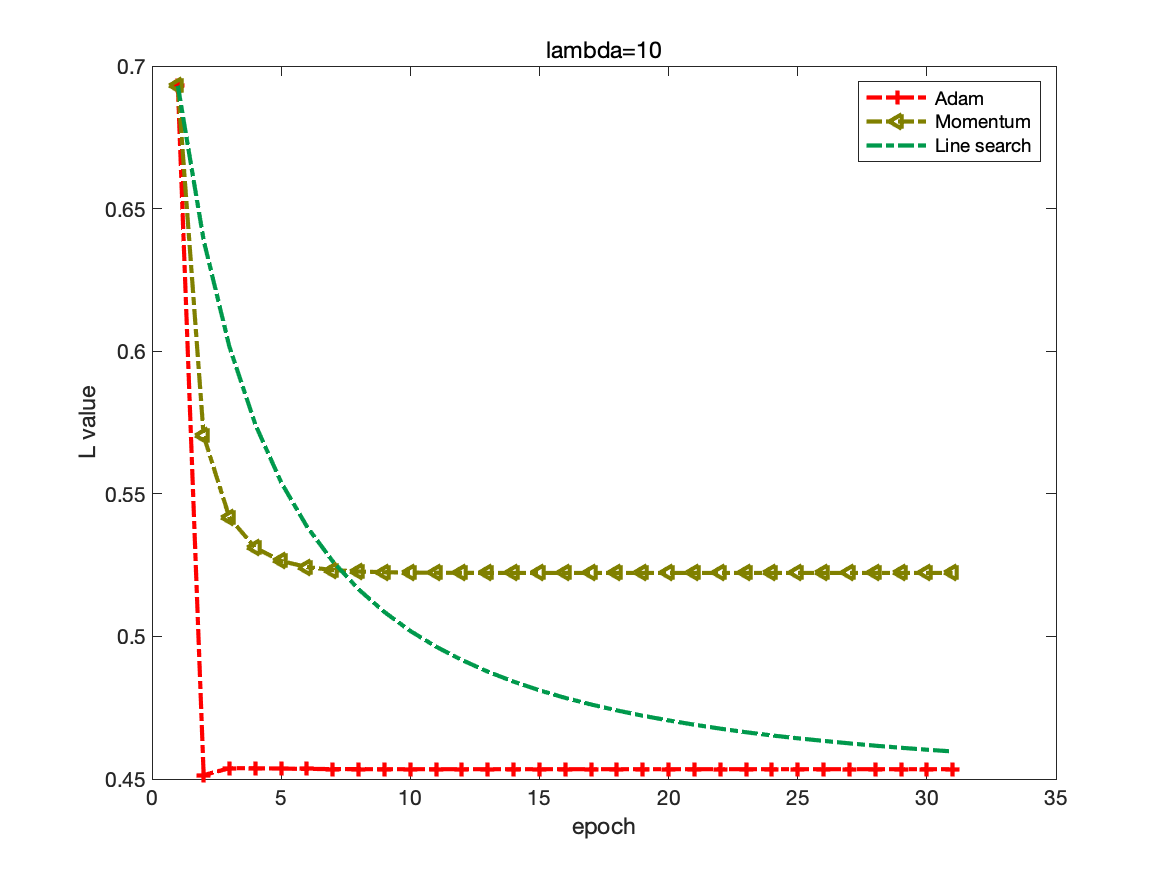
\includegraphics[width=1\linewidth]{./fig/fval_m1}
%	\end{minipage}
%%}
%%	\subfigure[gradient norm]{
%	\begin{minipage}{0.48\linewidth}
%		\centering
%		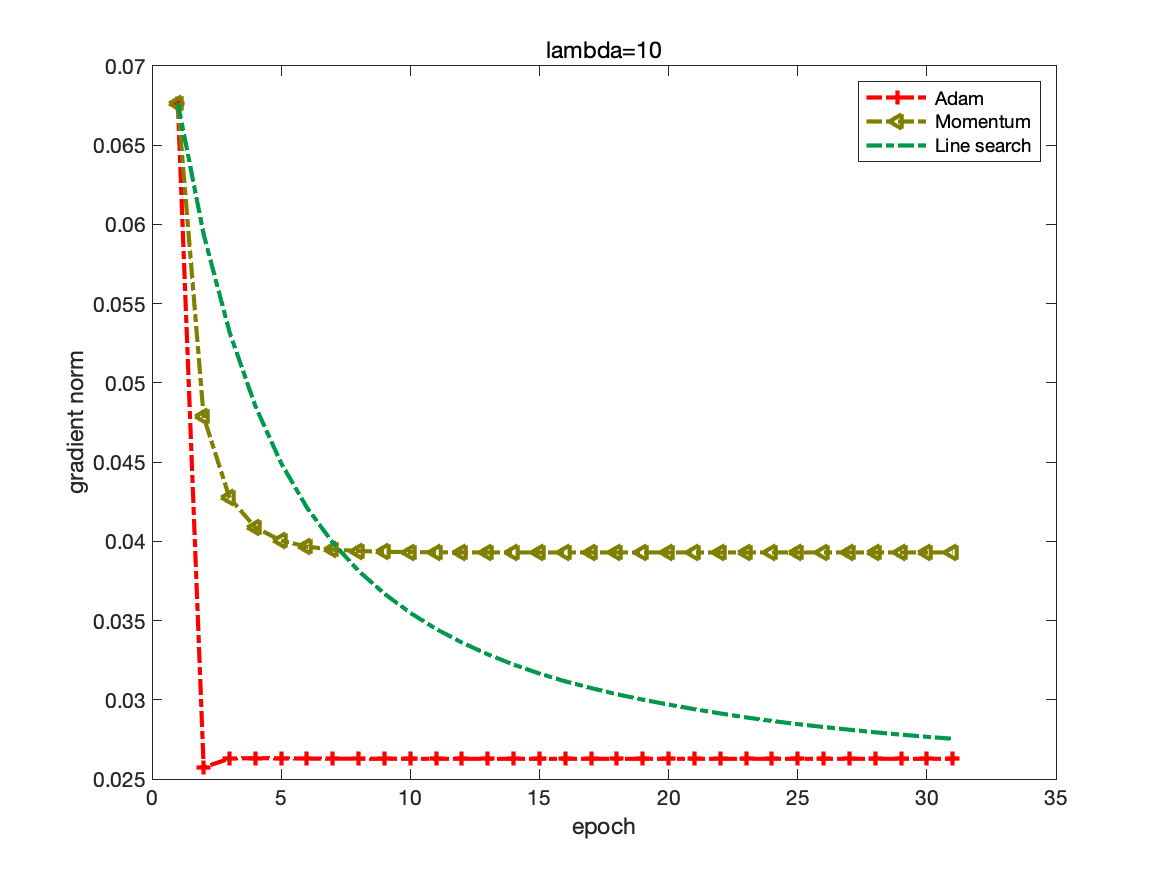
\includegraphics[width=1\linewidth]{./fig/gnorm_m1}
%	\end{minipage}
%%}
%%\subfigure[Testing error]{
%\begin{minipage}{0.48\linewidth}
%	\centering
%	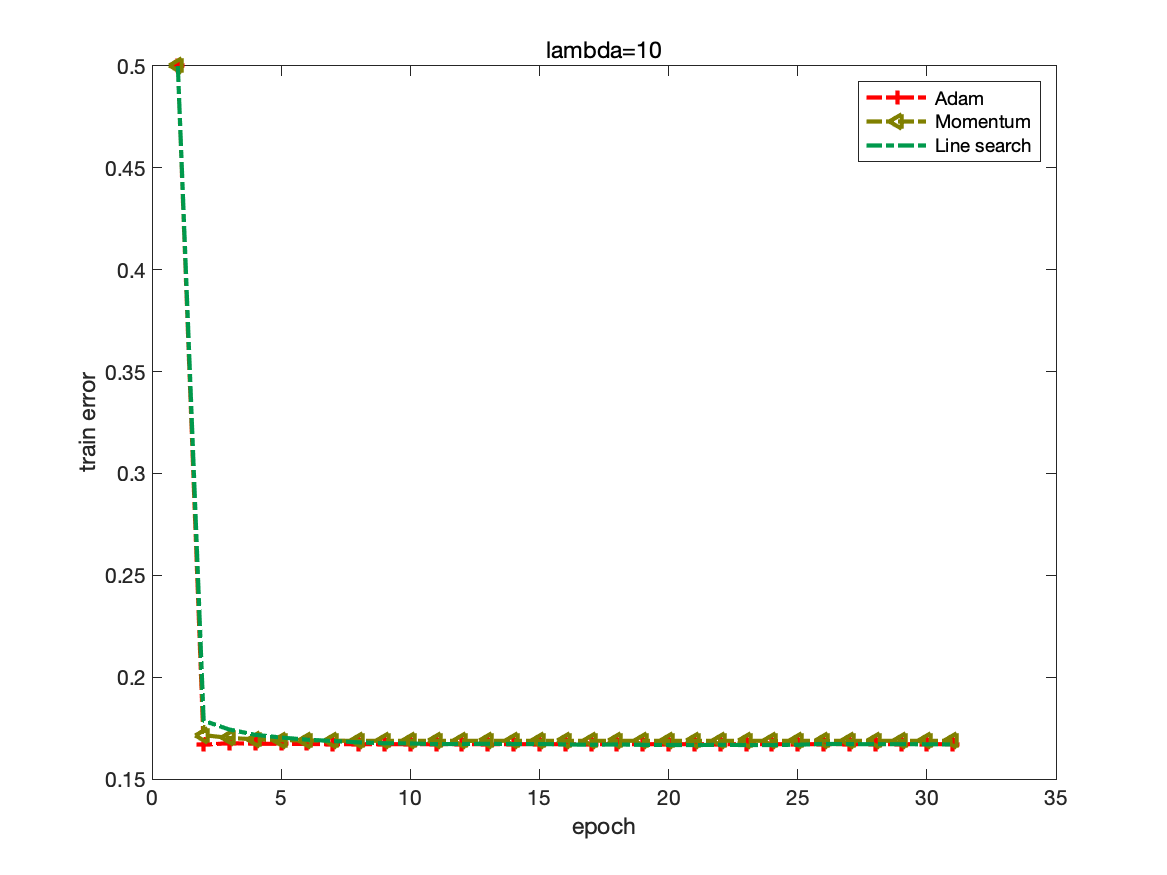
\includegraphics[width=1\linewidth]{./fig/err_m1}
%\end{minipage}
%%}
%\caption{Results on MNIST when $\lambda=10$
%\end{figure}
\begin{figure}[H]
	\begin{minipage}{0.33\linewidth}
		\centering
		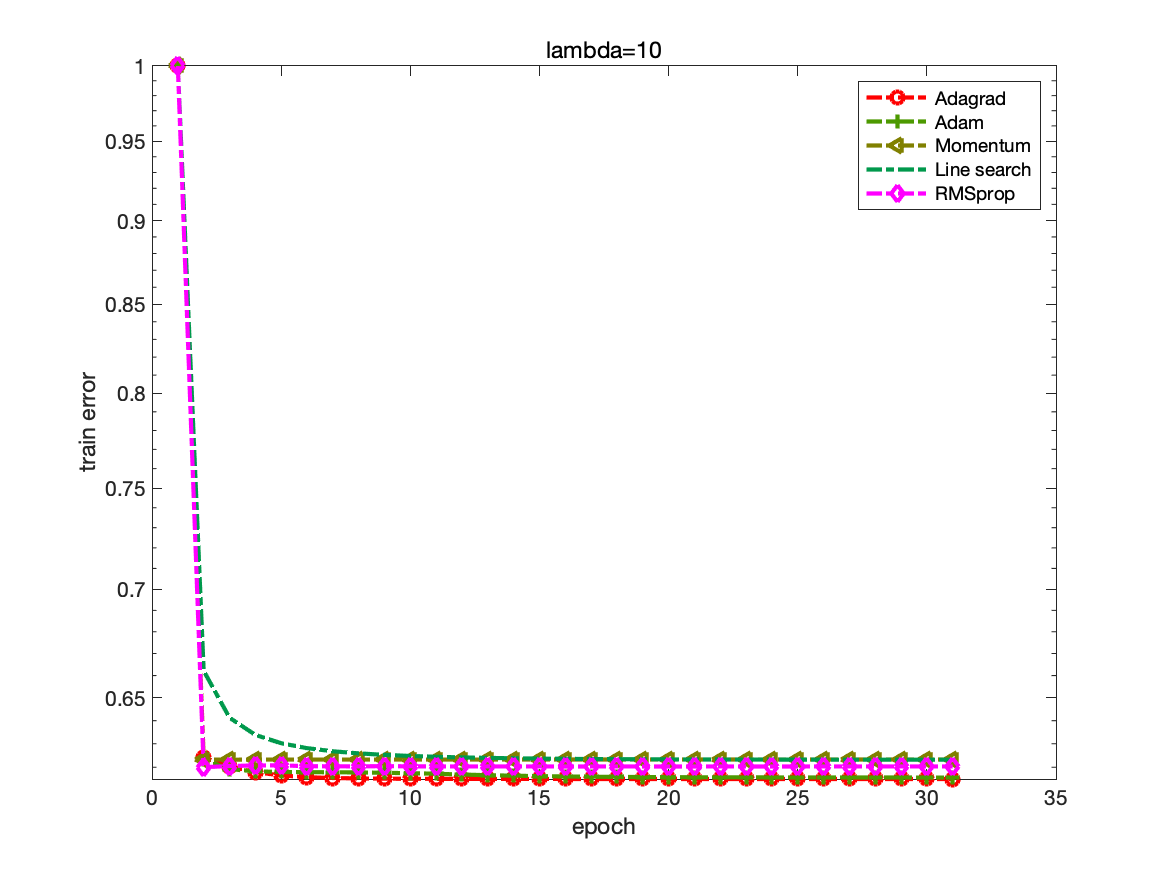
\includegraphics[width=1\linewidth]{./fig/fval_c1}
		\caption{Training errer}
	\end{minipage}
	\begin{minipage}{0.33\linewidth}
		\centering
		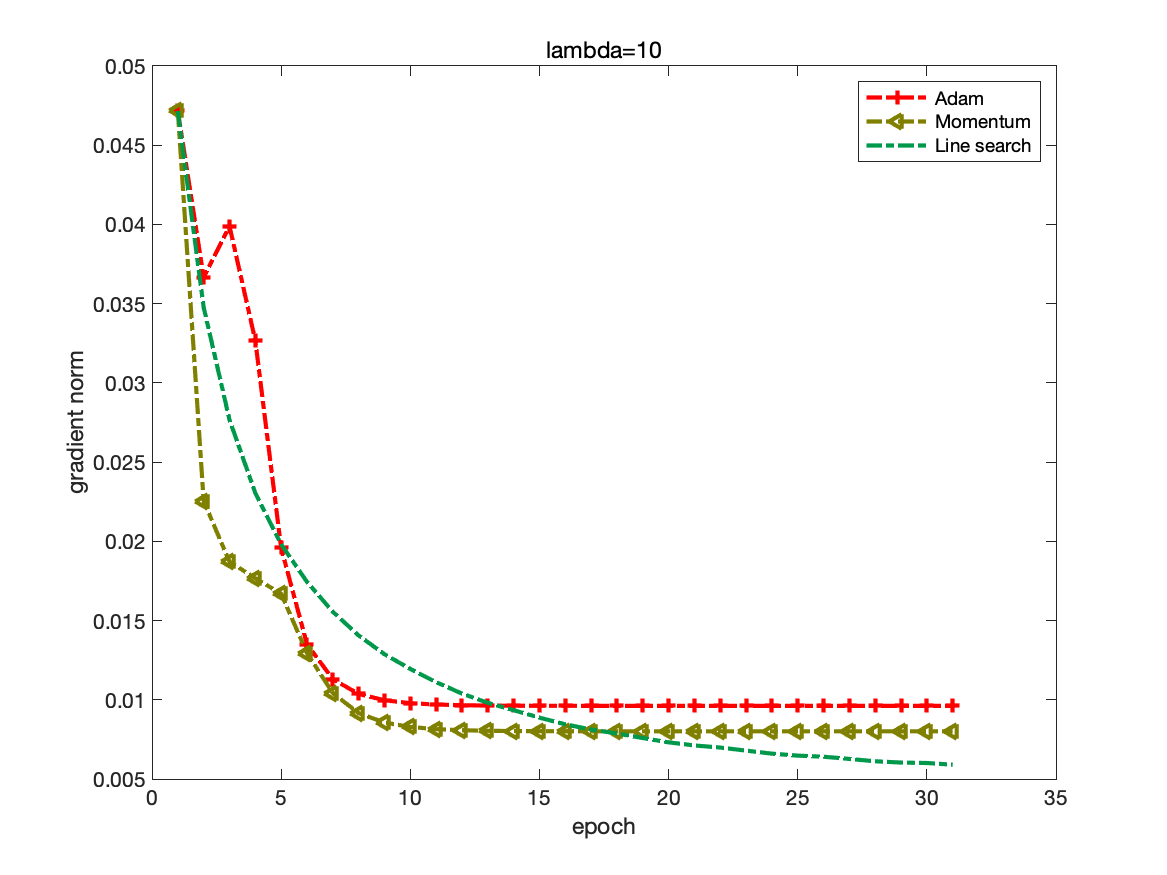
\includegraphics[width=1\linewidth]{./fig/gnorm_c1}
		\caption{gradient norm}
	\end{minipage}
	\begin{minipage}{0.33\linewidth}
		\centering
		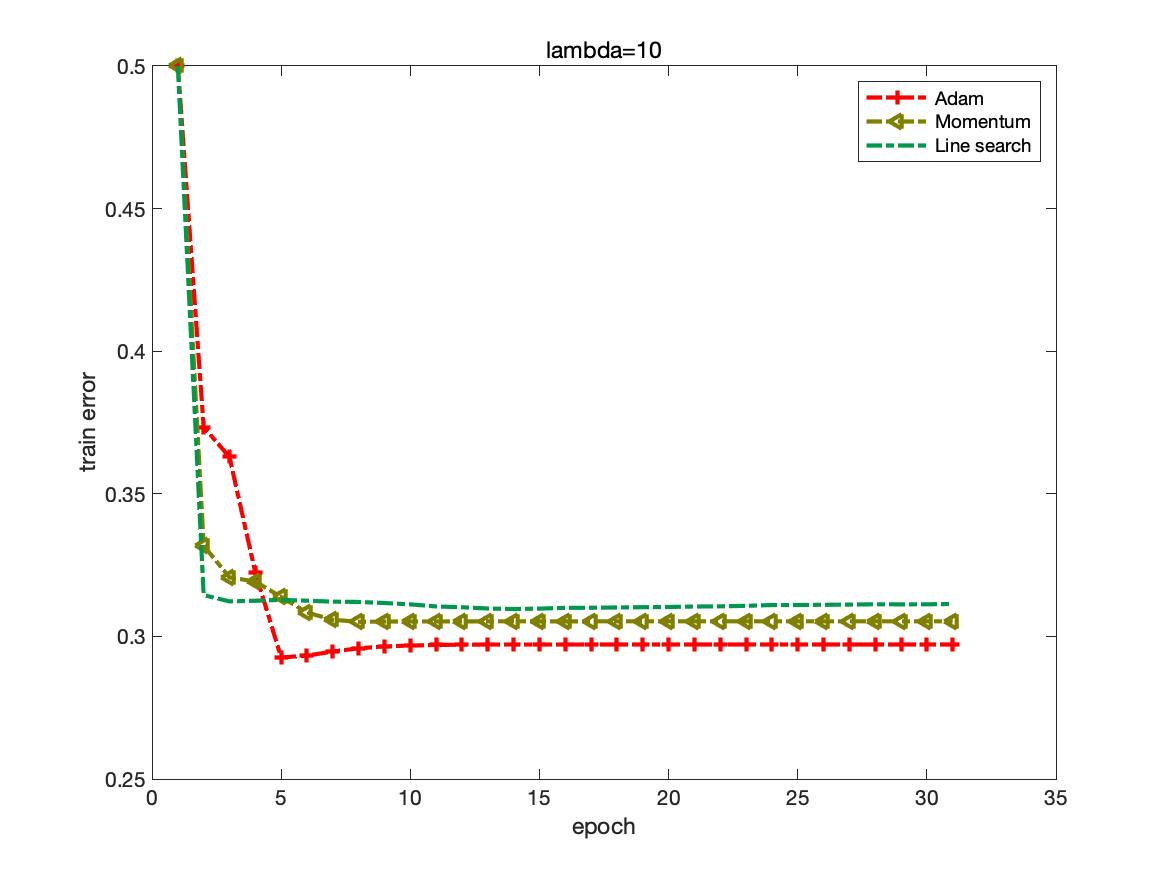
\includegraphics[width=1\linewidth]{./fig/err_c1}
		\caption{Testing error}
	\end{minipage}
	\caption*{Results on Covtype when $\lambda=10$}
\end{figure}
\begin{figure}[H]
	\begin{minipage}{0.33\linewidth}
		\centering
		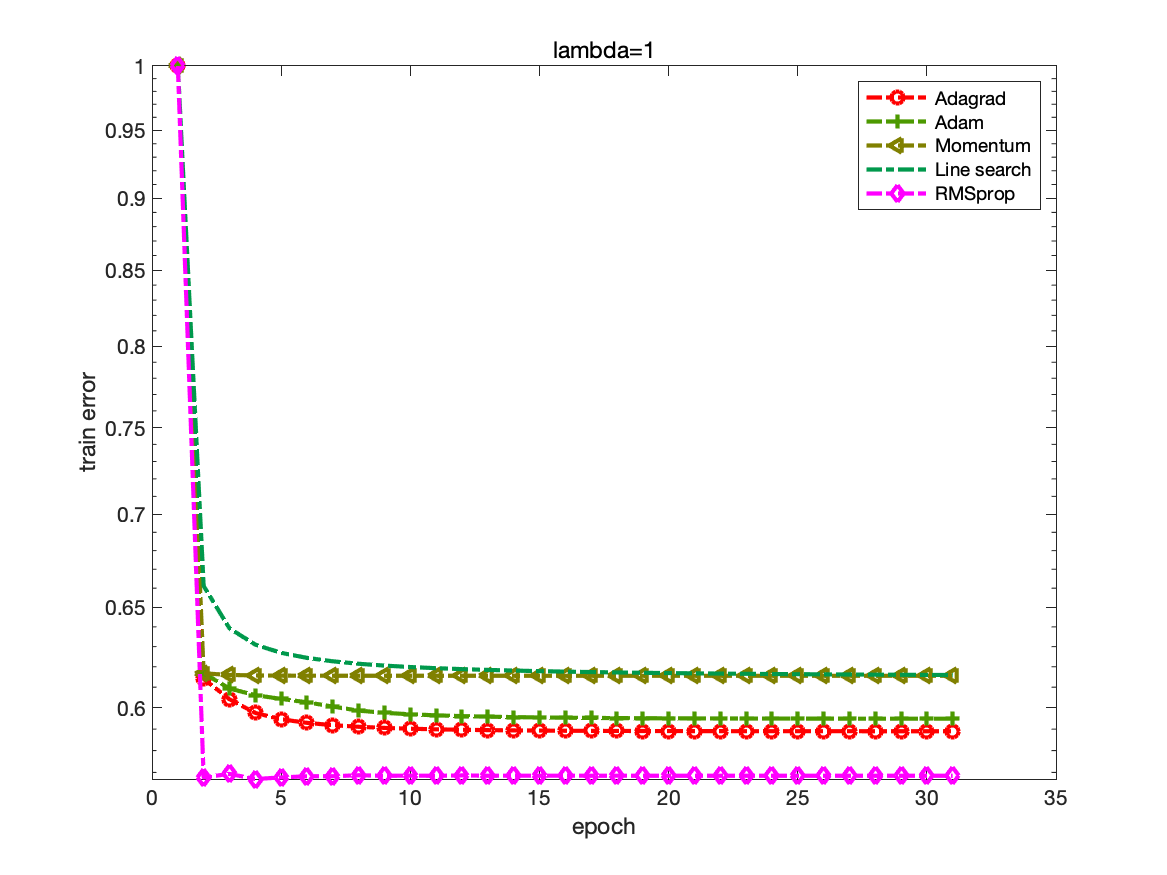
\includegraphics[width=1\linewidth]{./fig/fval_c2}
		\caption{Training errer}
	\end{minipage}
	\begin{minipage}{0.33\linewidth}
		\centering
		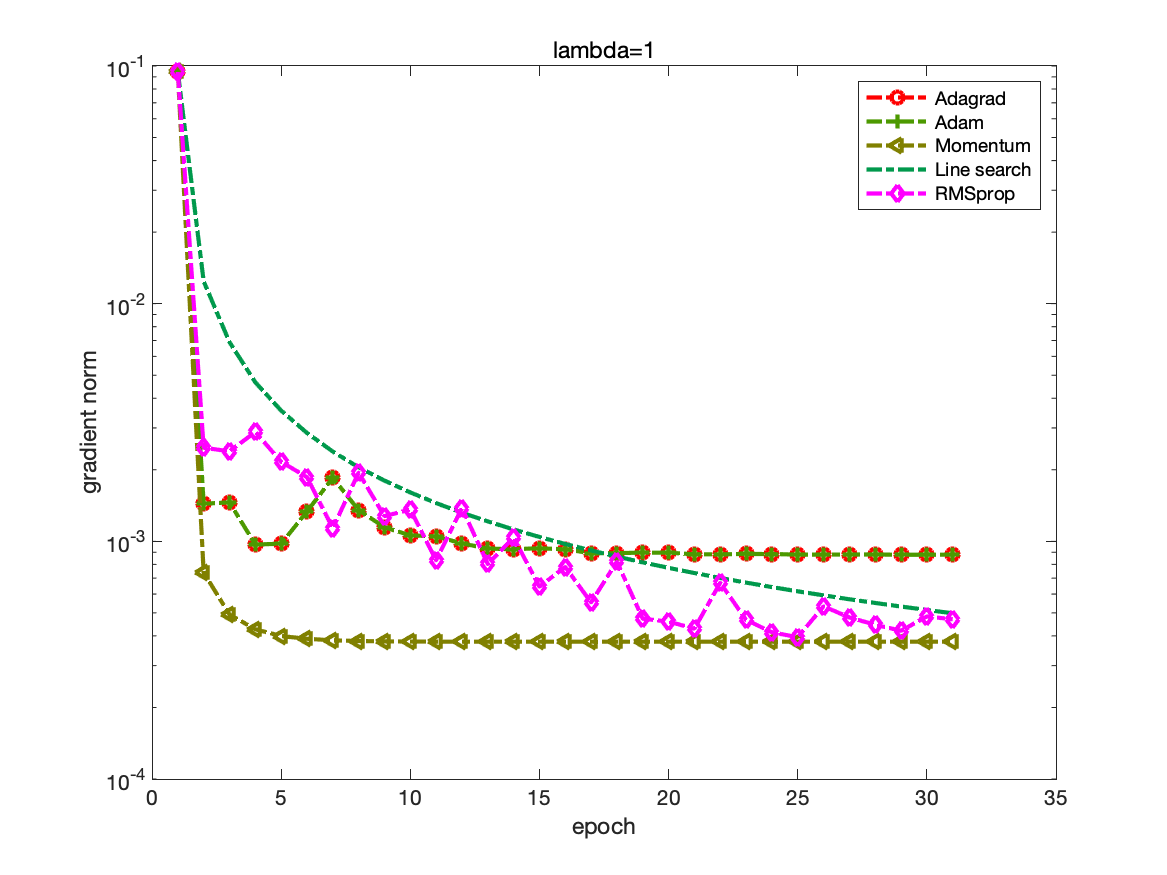
\includegraphics[width=1\linewidth]{./fig/gnorm_c2}
		\caption{gradient norm}
	\end{minipage}
	\begin{minipage}{0.33\linewidth}
		\centering
		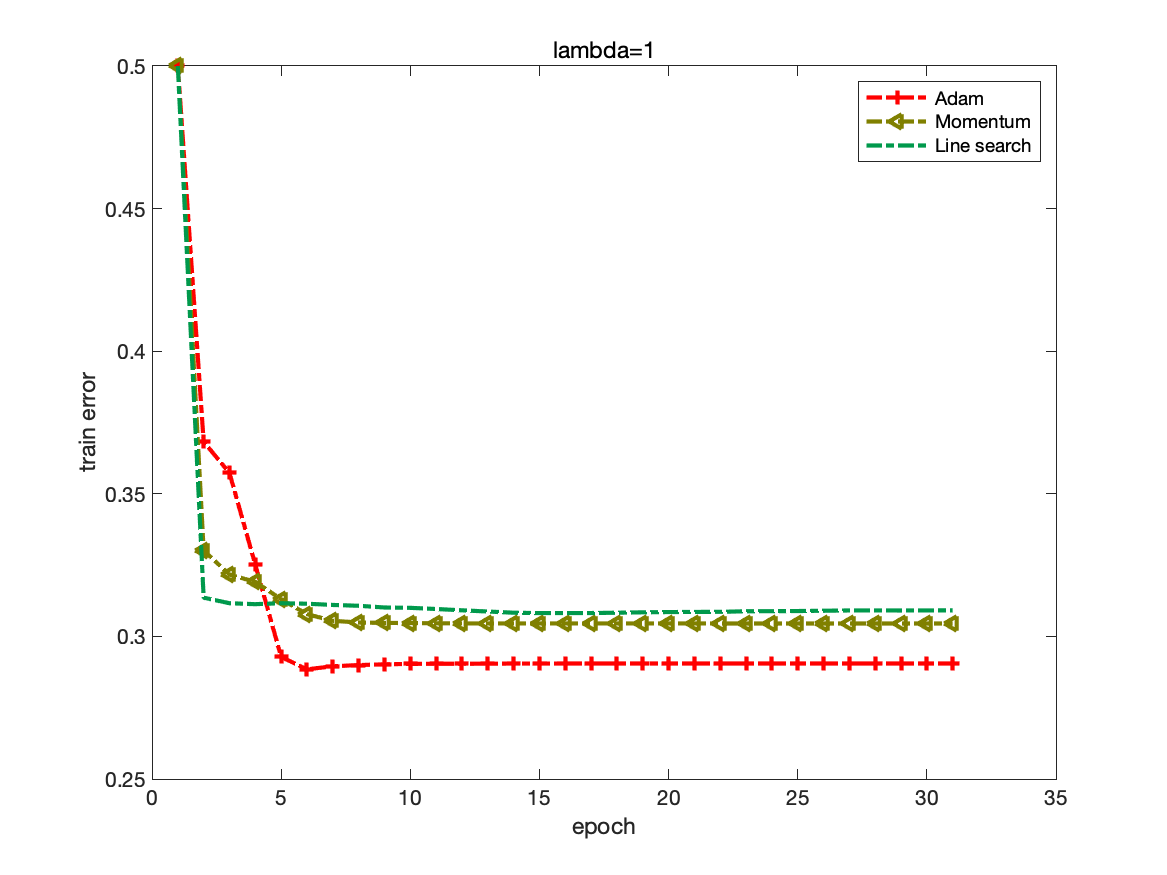
\includegraphics[width=1\linewidth]{./fig/err_c2}
		\caption{Testing error}
	\end{minipage}
	\caption*{Results on Covtype when $\lambda=1$}
\end{figure}
\begin{figure}[H]
	\begin{minipage}{0.33\linewidth}
		\centering
		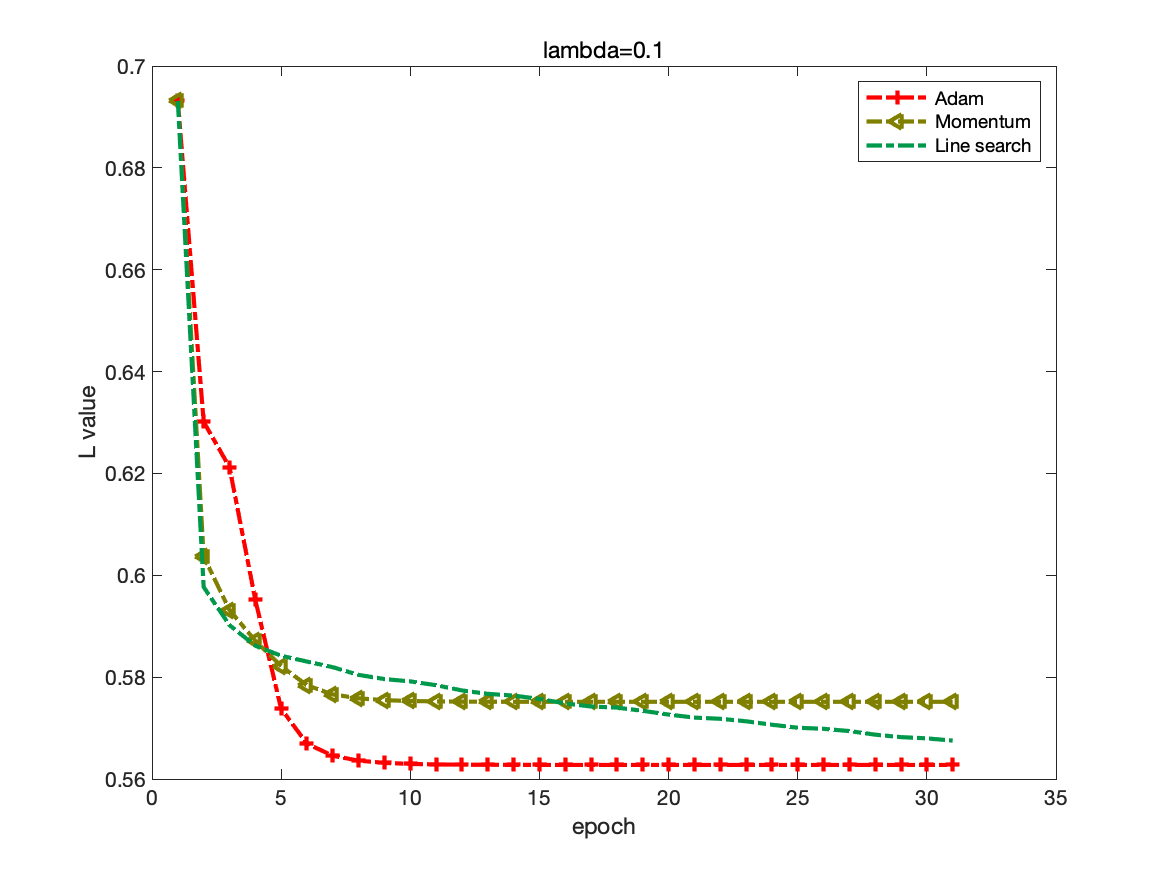
\includegraphics[width=1\linewidth]{./fig/fval_c3}
		\caption{Training errer}
	\end{minipage}
	\begin{minipage}{0.33\linewidth}
		\centering
		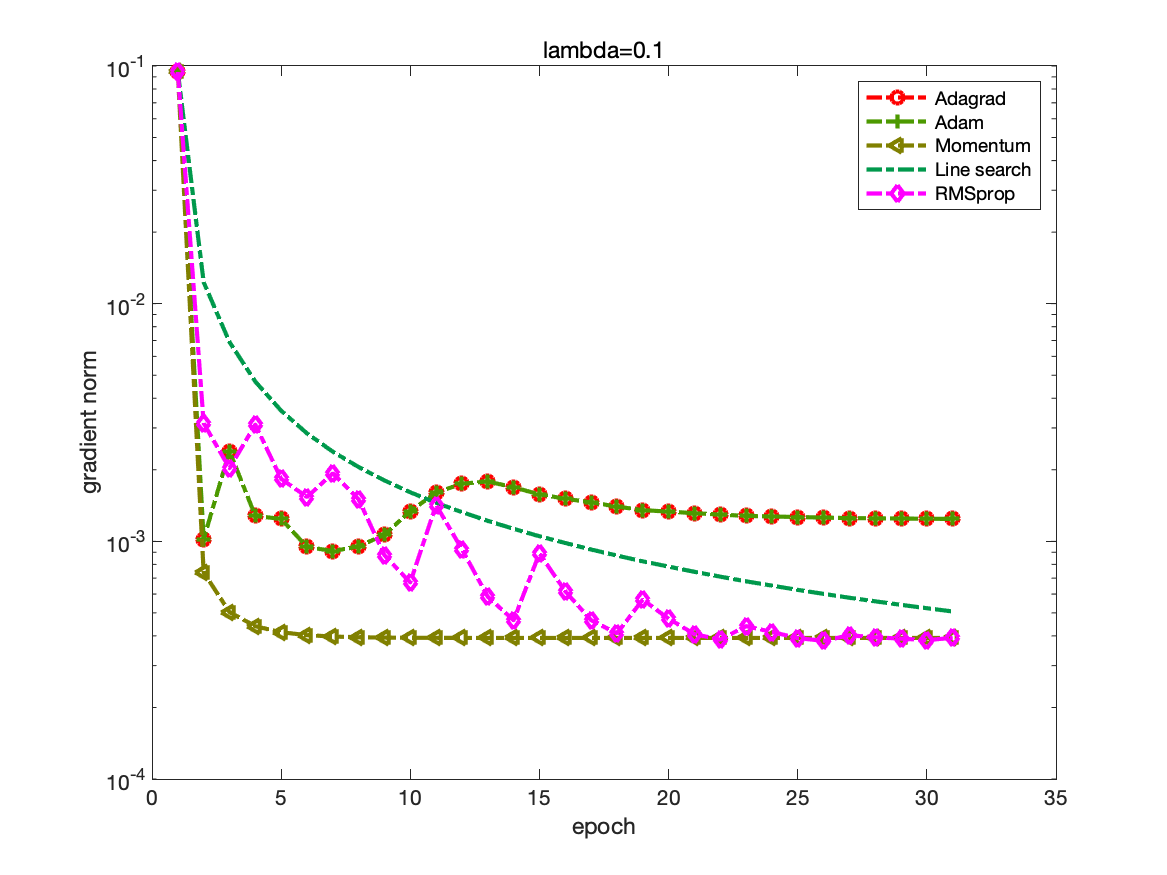
\includegraphics[width=1\linewidth]{./fig/gnorm_c3}
		\caption{gradient norm}
	\end{minipage}
	\begin{minipage}{0.33\linewidth}
		\centering
		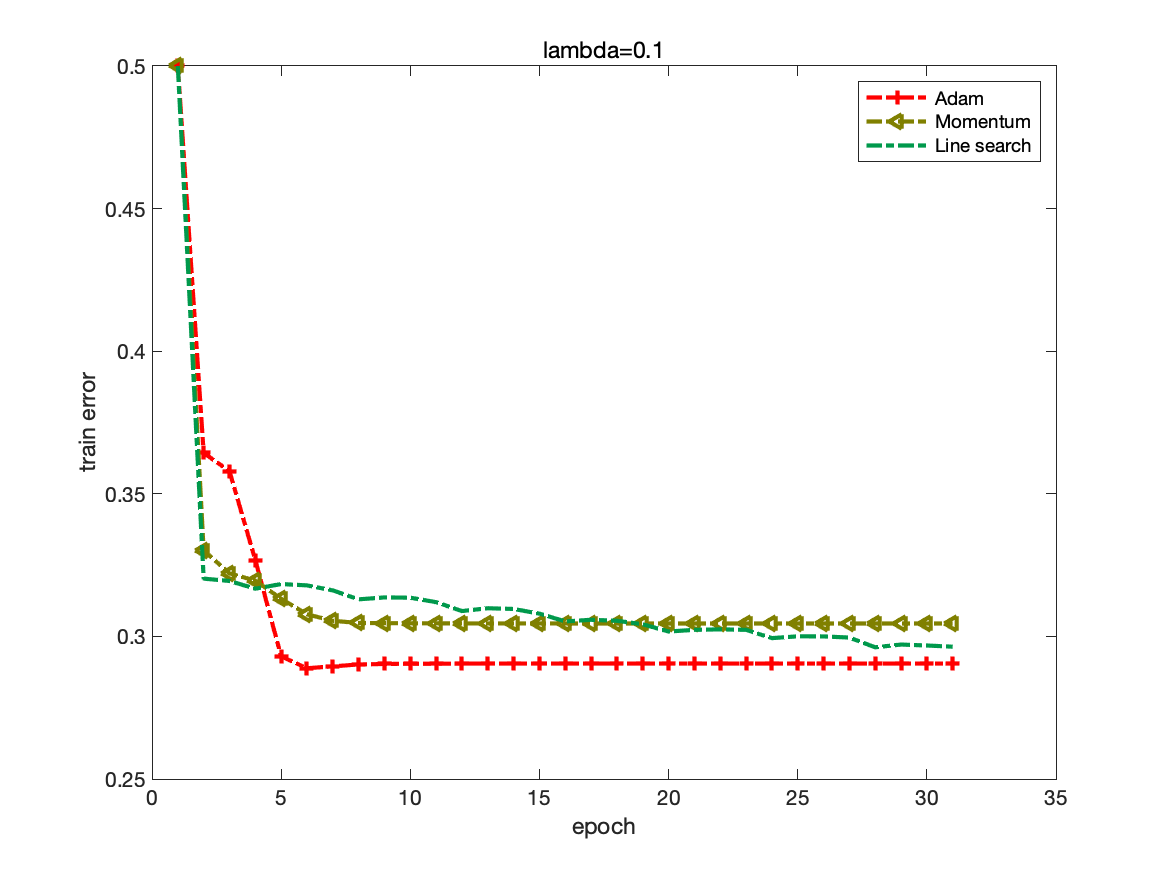
\includegraphics[width=1\linewidth]{./fig/err_c3}
		\caption{Testing error}
	\end{minipage}
	\caption*{Results on Covtype when $\lambda=0.1$}
\end{figure}
\begin{figure}[H]
	\begin{minipage}{0.33\linewidth}
		\centering
		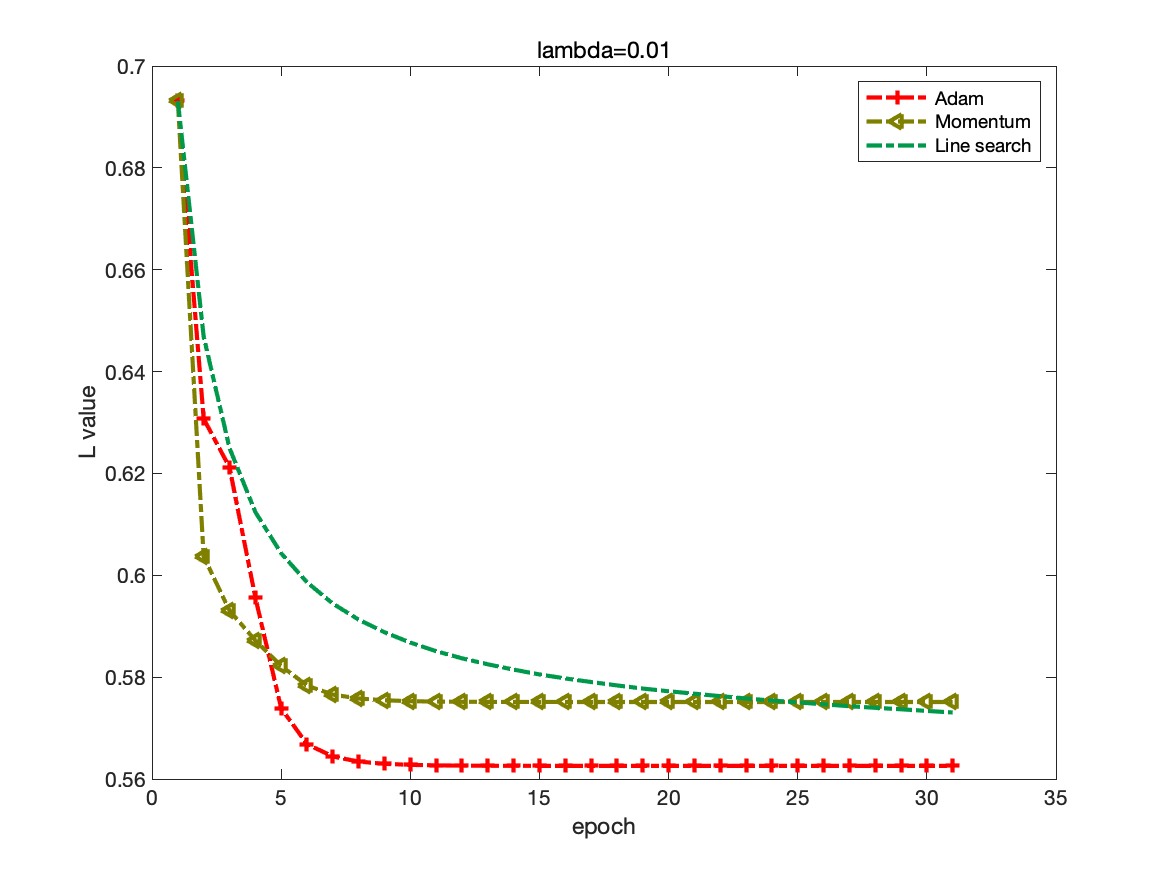
\includegraphics[width=1\linewidth]{./fig/fval_c4}
		\caption{Training errer}
	\end{minipage}
	\begin{minipage}{0.33\linewidth}
		\centering
		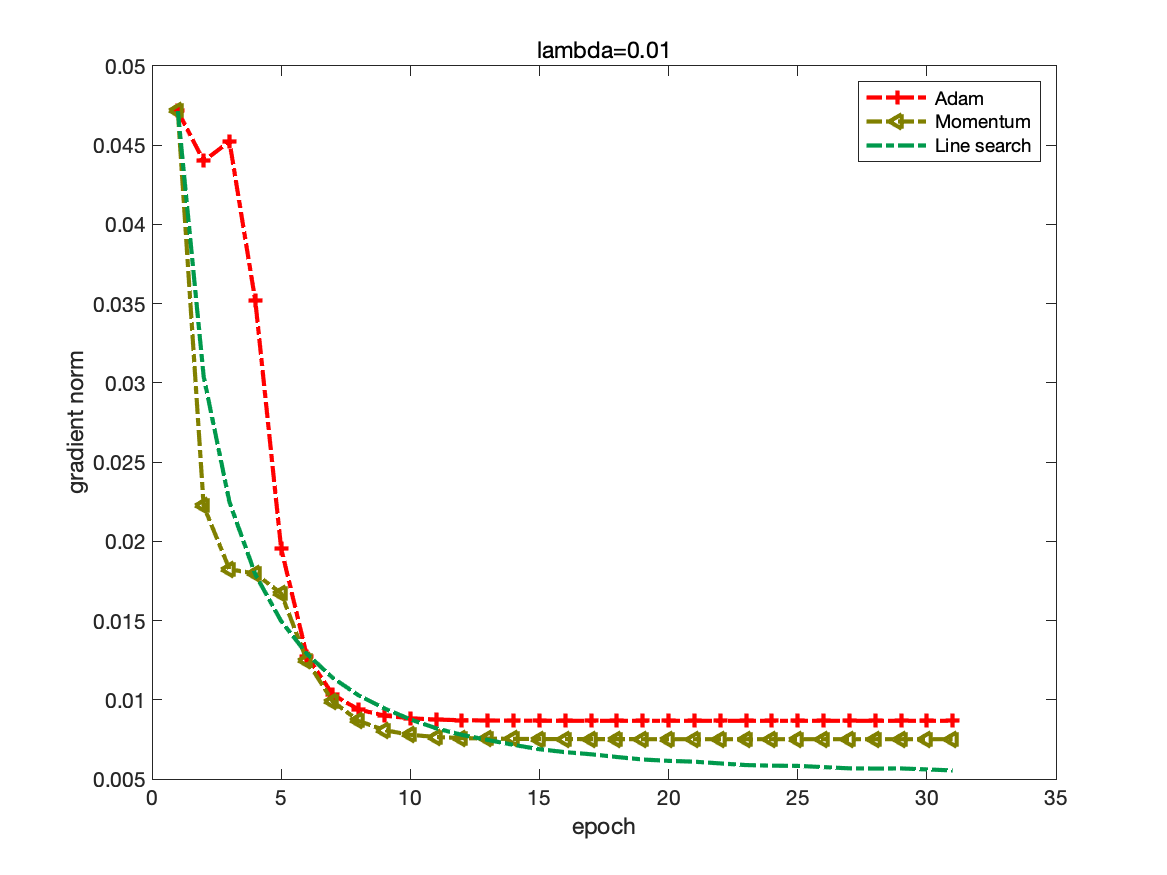
\includegraphics[width=1\linewidth]{./fig/gnorm_c4}
		\caption{gradient norm}
	\end{minipage}
	\begin{minipage}{0.33\linewidth}
		\centering
		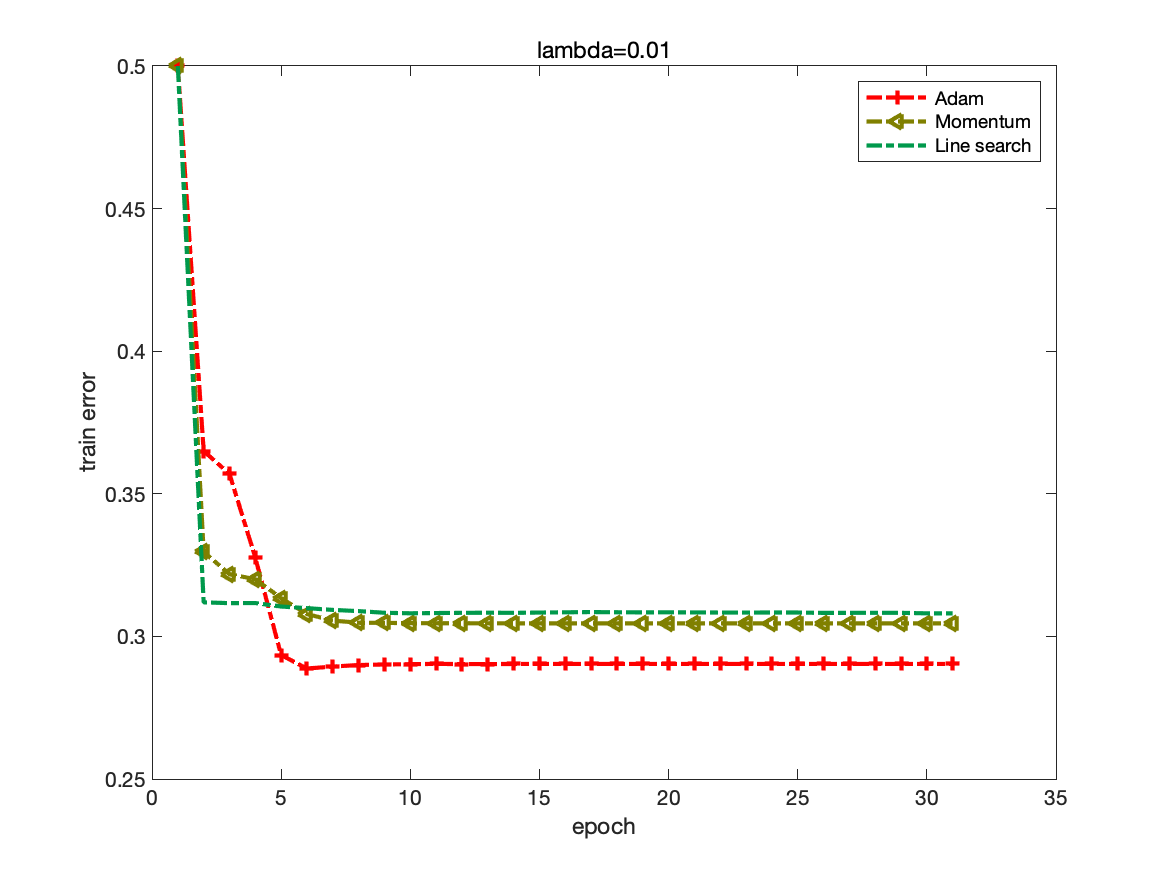
\includegraphics[width=1\linewidth]{./fig/err_c4}
		\caption{Testing error}
	\end{minipage}
	\caption*{Results on Covtype when $\lambda=0.01$}
\end{figure}
\begin{figure}[H]
	\begin{minipage}{0.33\linewidth}
		\centering
		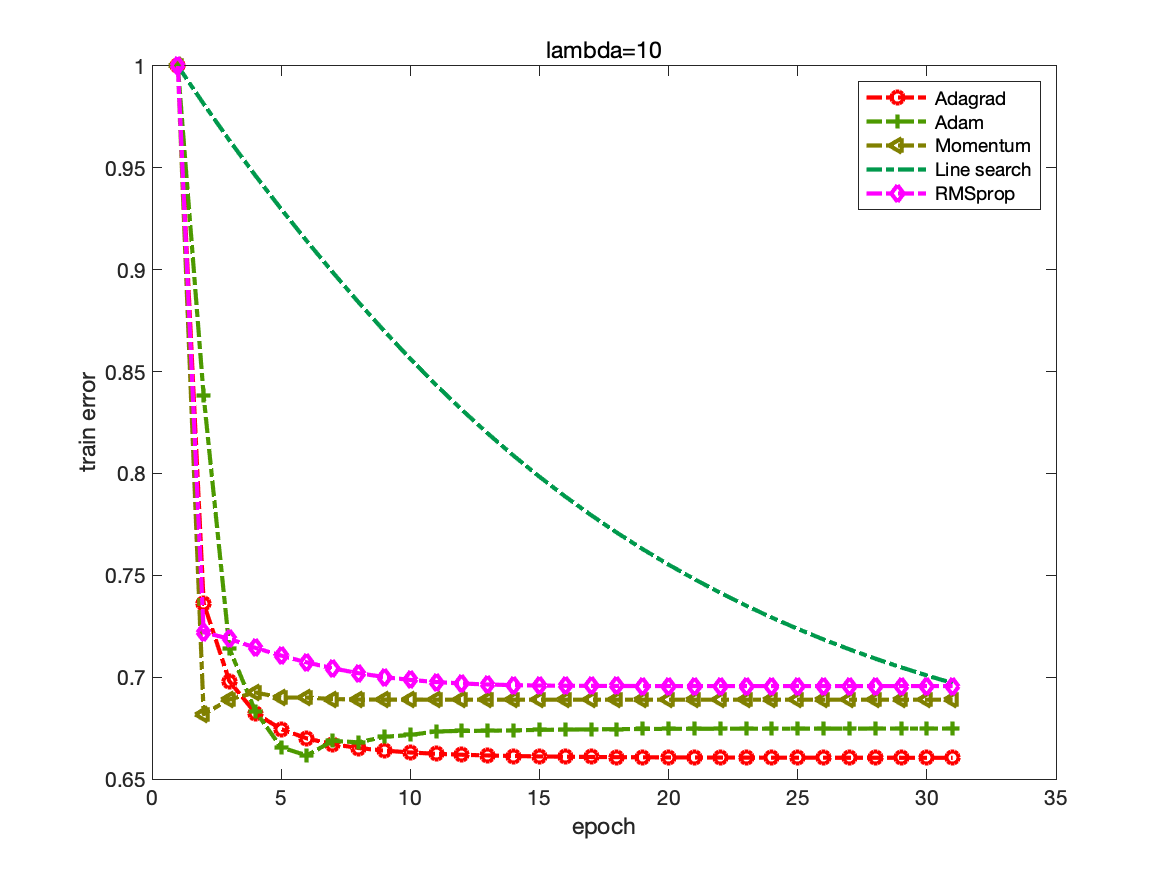
\includegraphics[width=1\linewidth]{./fig/fval_g1}
		\caption{Training errer}
	\end{minipage}
	\begin{minipage}{0.33\linewidth}
		\centering
		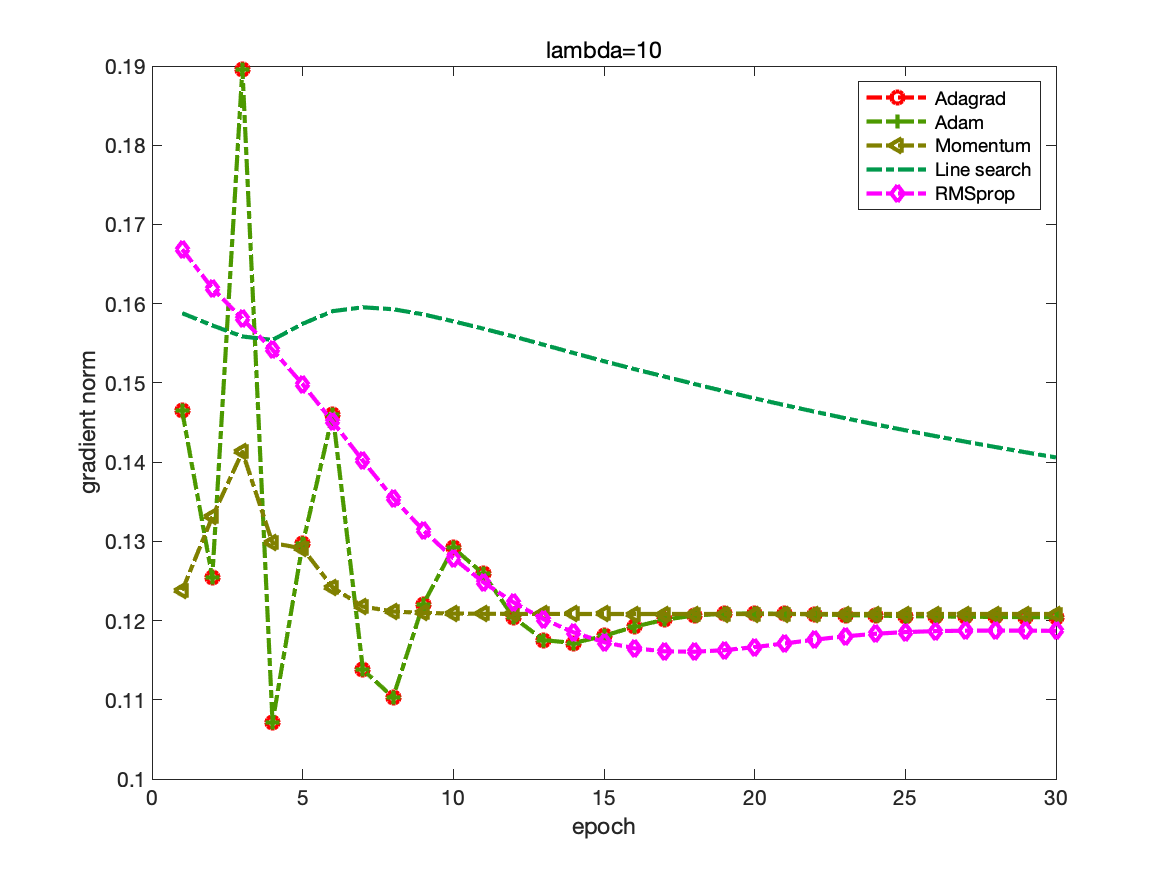
\includegraphics[width=1\linewidth]{./fig/gnorm_g1}
		\caption{gradient norm}
	\end{minipage}
	\begin{minipage}{0.33\linewidth}
		\centering
		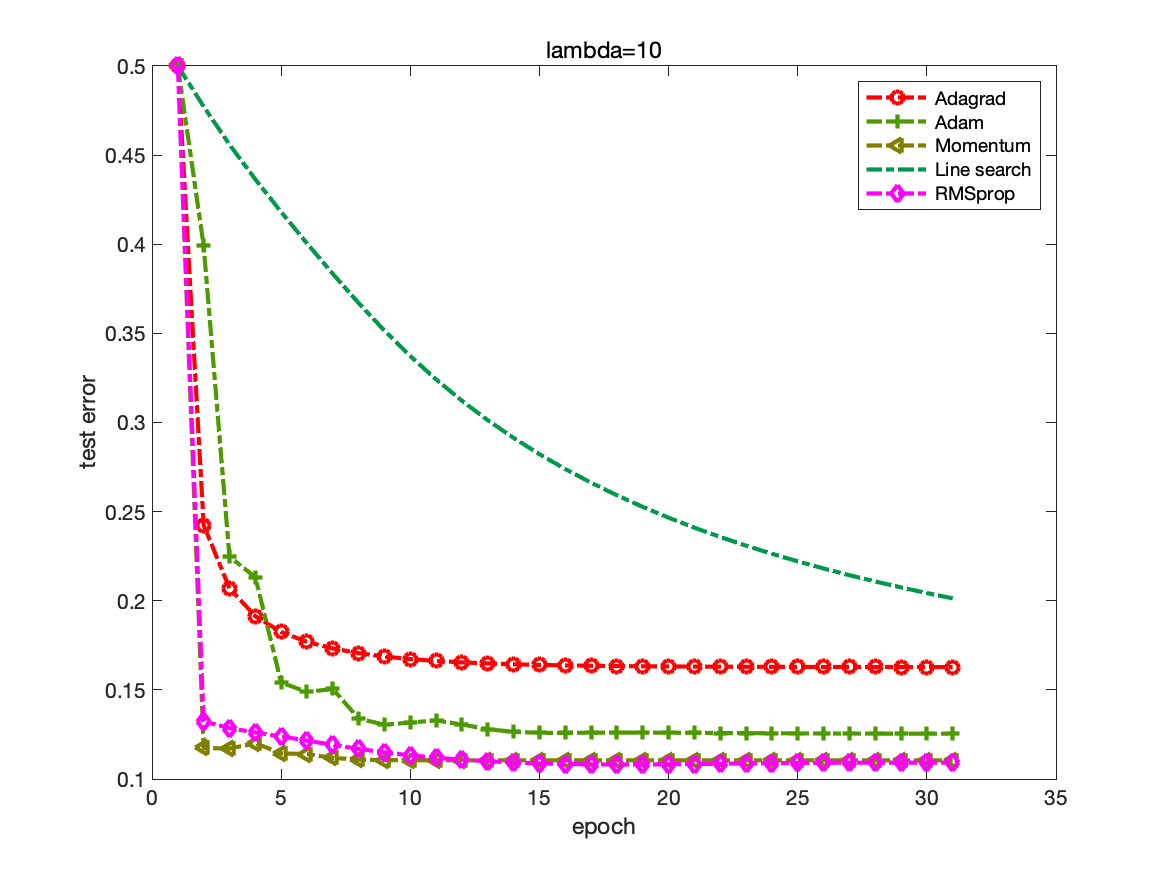
\includegraphics[width=1\linewidth]{./fig/err_g1}
		\caption{Testing error}
	\end{minipage}
\caption*{Results on Gisette when $\lambda=10$}
\end{figure}
\begin{figure}[H]
\begin{minipage}{0.33\linewidth}
	\centering
	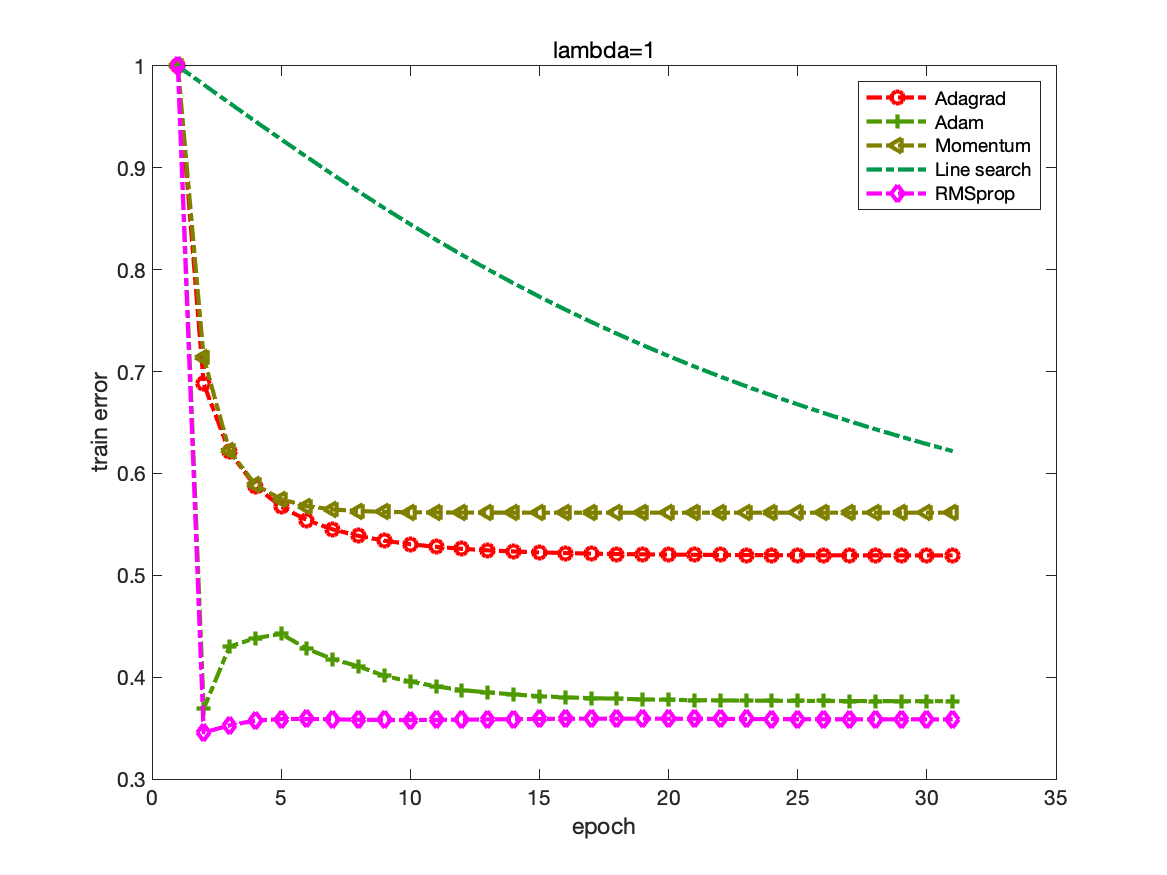
\includegraphics[width=1\linewidth]{./fig/fval_g2}
	\caption{Training errer}
\end{minipage}
\begin{minipage}{0.33\linewidth}
	\centering
	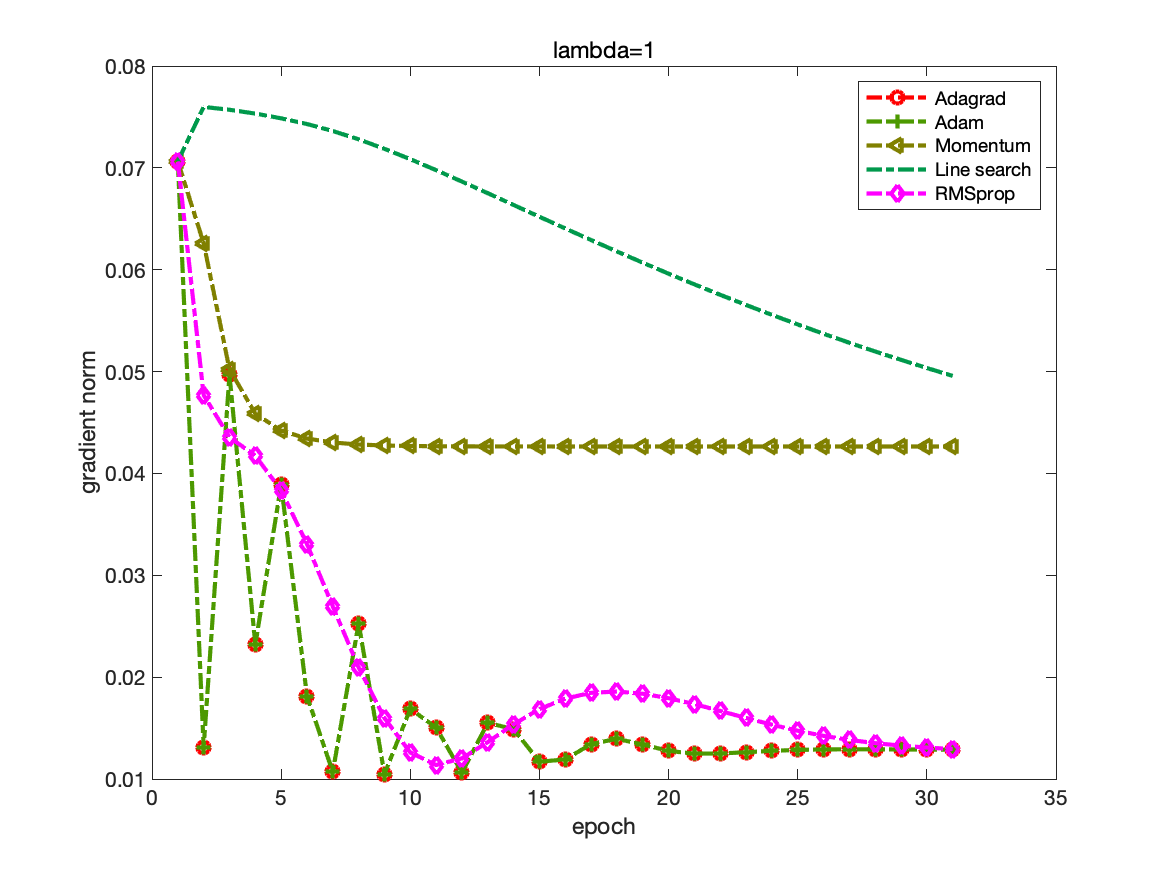
\includegraphics[width=1\linewidth]{./fig/gnorm_g2}
	\caption{gradient norm}
\end{minipage}
\begin{minipage}{0.33\linewidth}
	\centering
	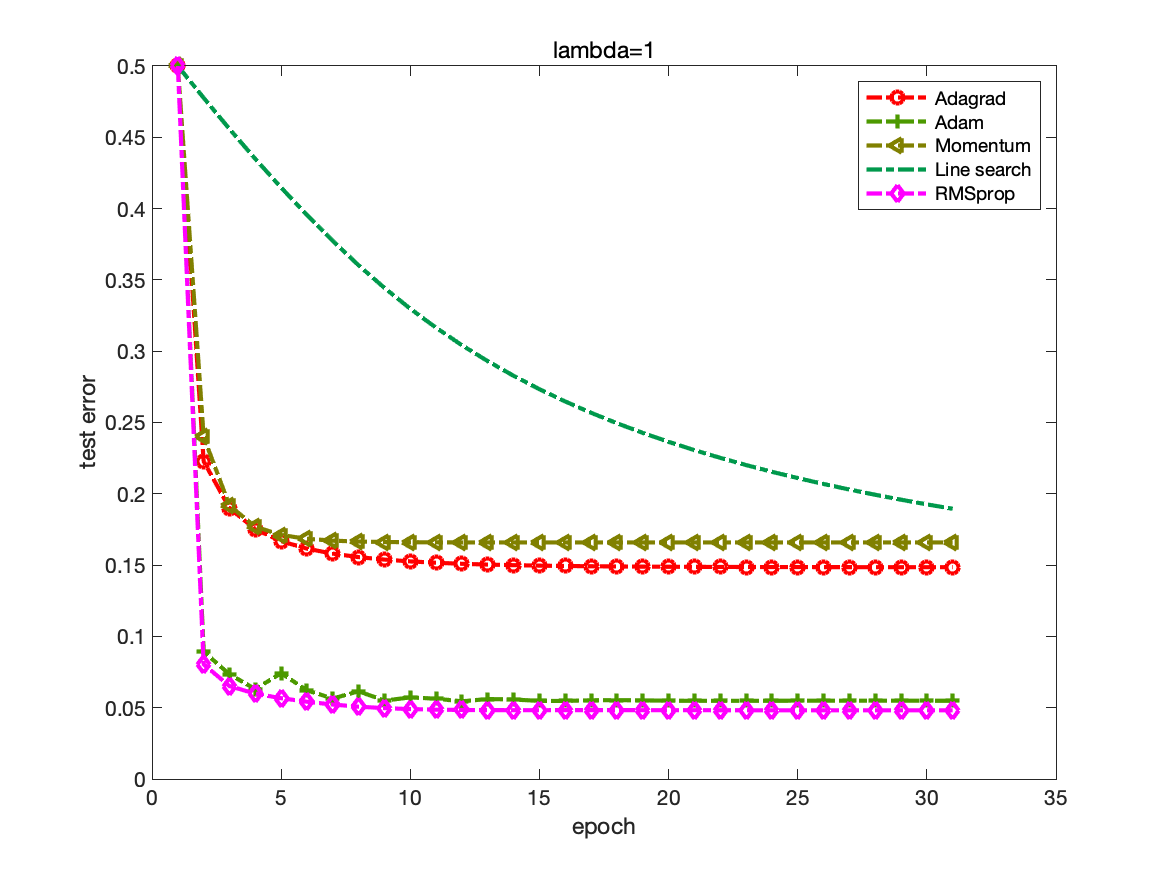
\includegraphics[width=1\linewidth]{./fig/err_g2}
	\caption{Testing error}
\end{minipage}
\caption*{Results on Gisette when $\lambda=1$}
\end{figure}
\begin{figure}[H]
\begin{minipage}{0.33\linewidth}
	\centering
	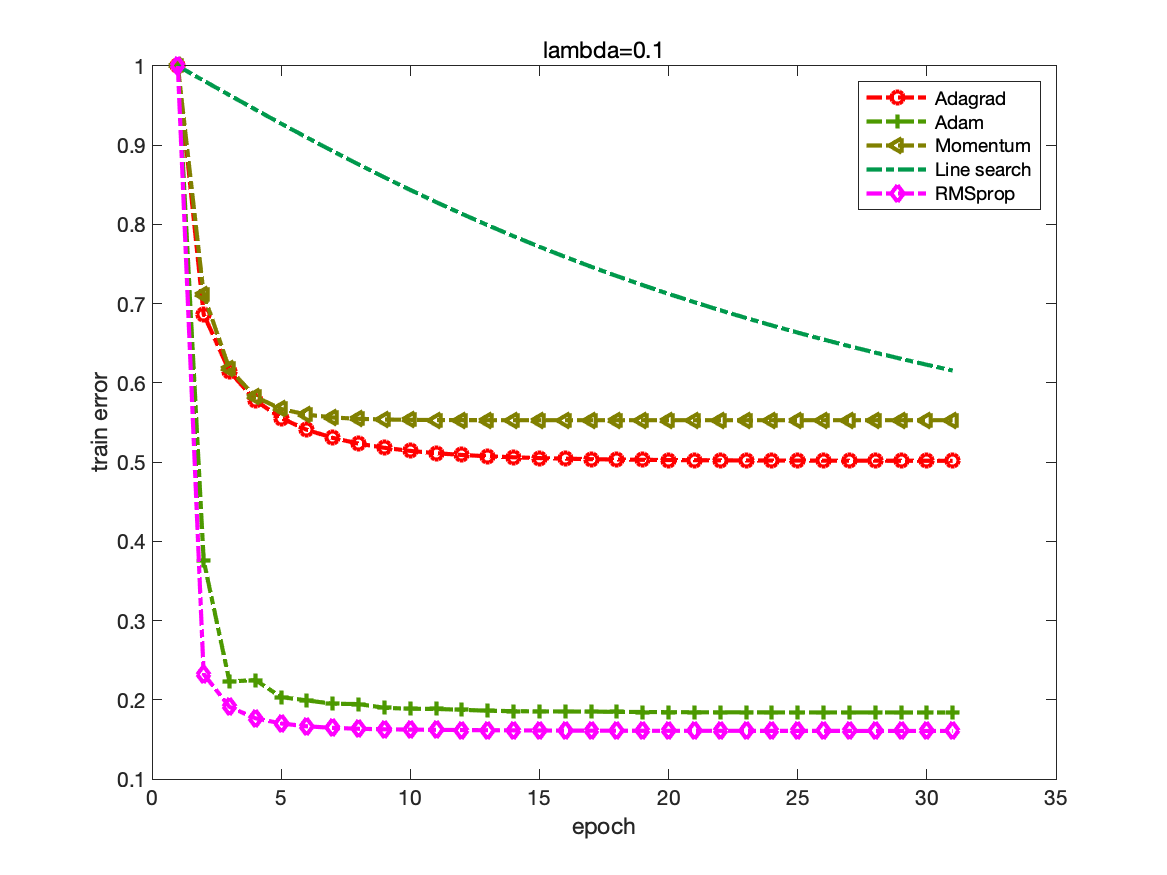
\includegraphics[width=1\linewidth]{./fig/fval_g3}
	\caption{Training errer}
\end{minipage}
\begin{minipage}{0.33\linewidth}
	\centering
	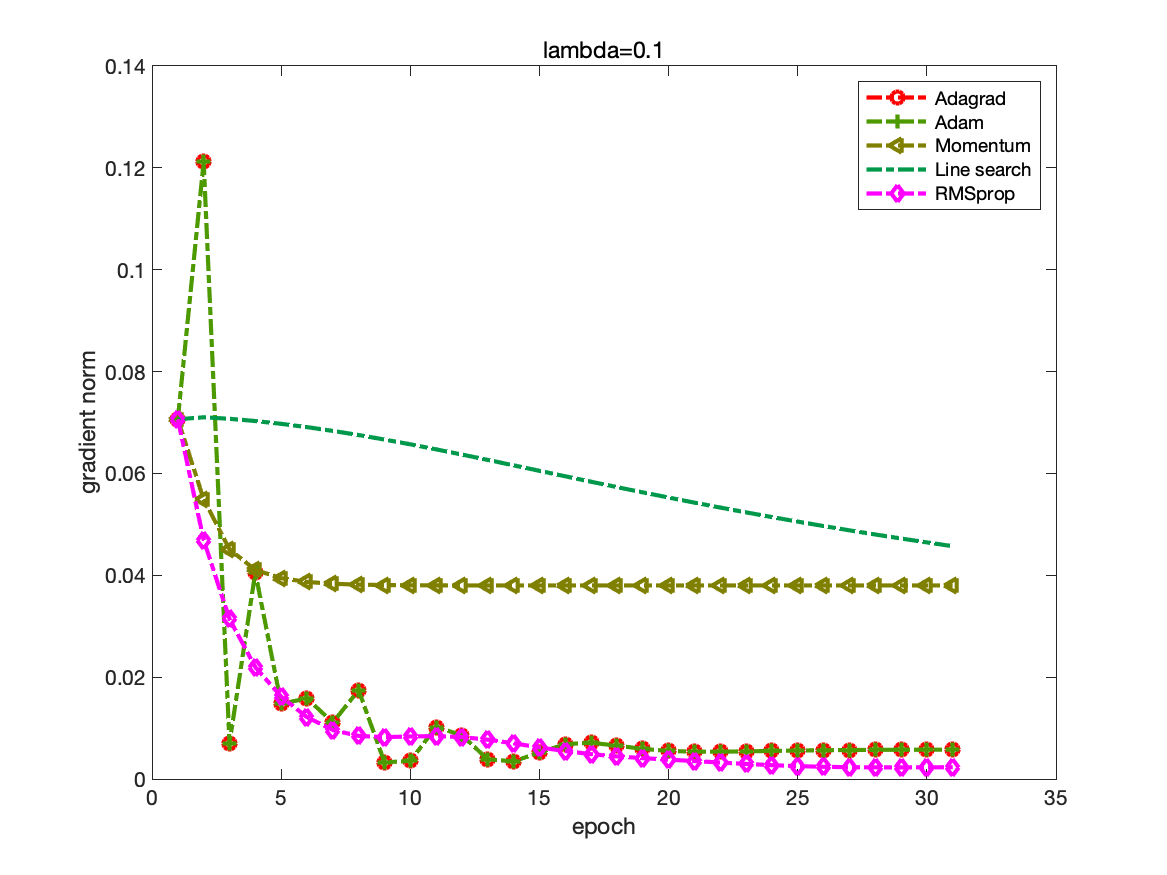
\includegraphics[width=1\linewidth]{./fig/gnorm_g3}
	\caption{gradient norm}
\end{minipage}
\begin{minipage}{0.33\linewidth}
	\centering
	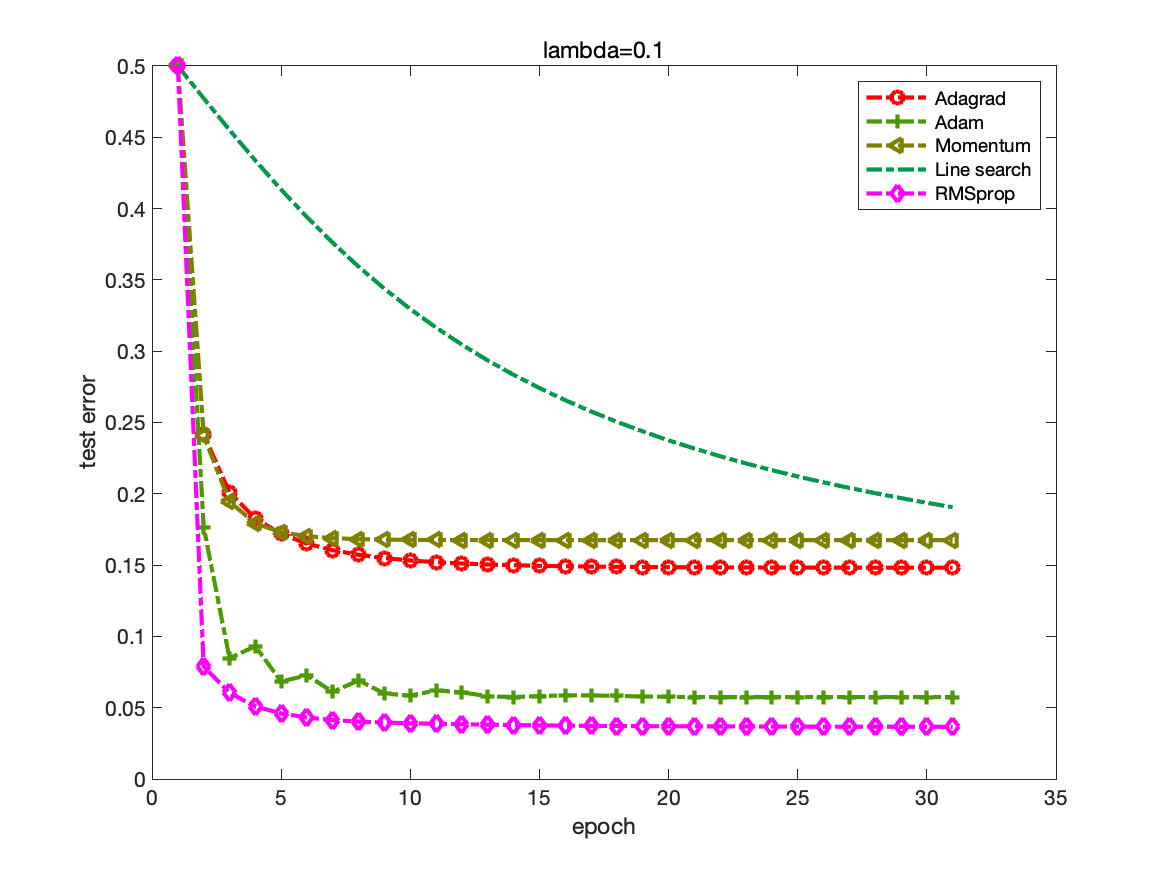
\includegraphics[width=1\linewidth]{./fig/err_g3}
	\caption{Testing error}
\end{minipage}
\caption*{Results on Gisette when $\lambda=0.1$}
\end{figure}
\begin{figure}[H]
\begin{minipage}{0.33\linewidth}
	\centering
	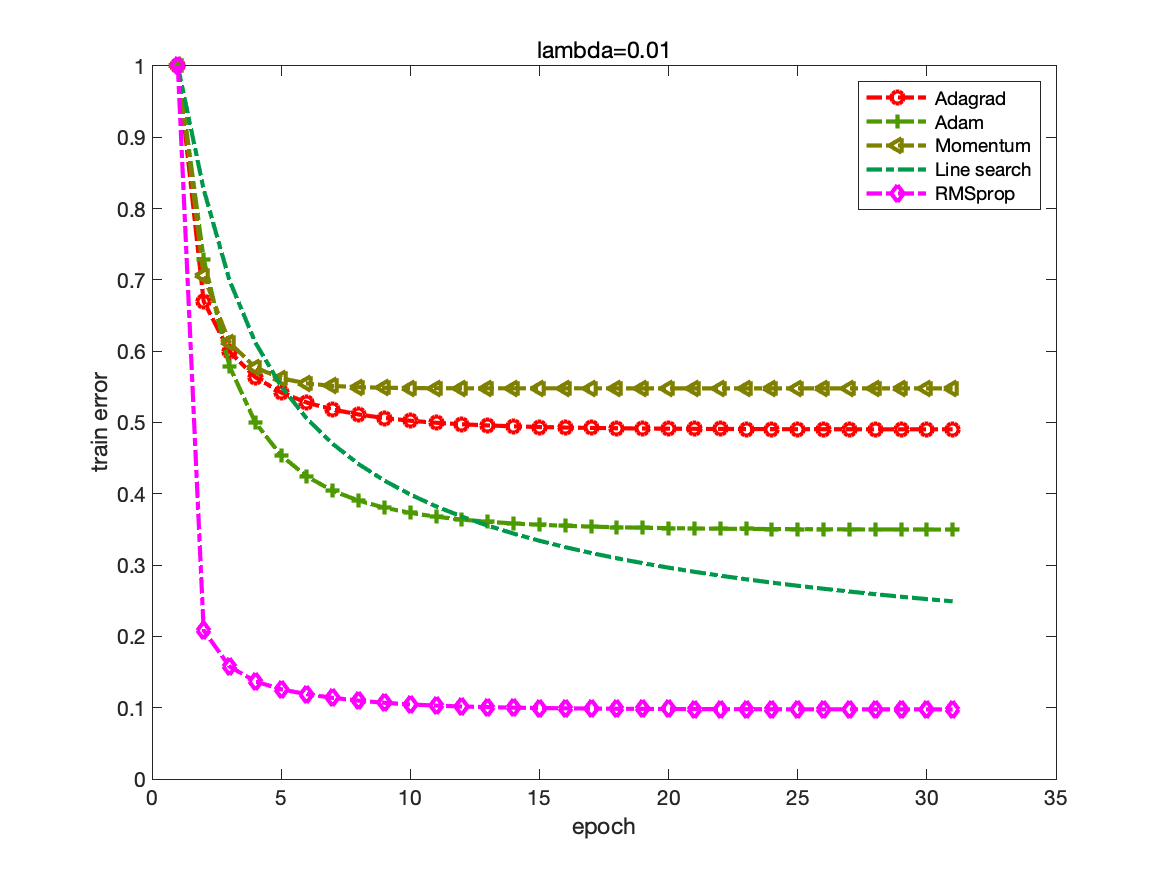
\includegraphics[width=1\linewidth]{./fig/fval_g4}
	\caption{Training errer}
\end{minipage}
\begin{minipage}{0.33\linewidth}
	\centering
	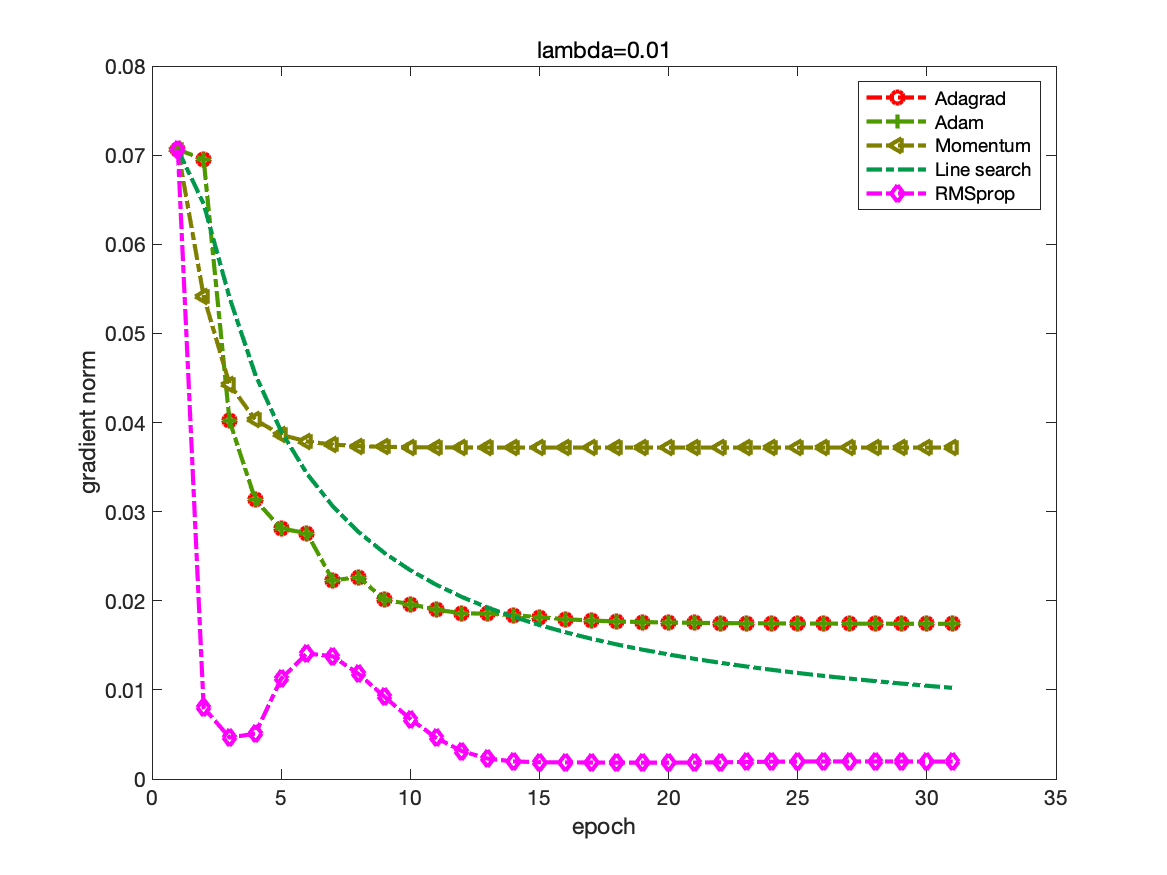
\includegraphics[width=1\linewidth]{./fig/gnorm_g4}
	\caption{gradient norm}
\end{minipage}
\begin{minipage}{0.33\linewidth}
	\centering
	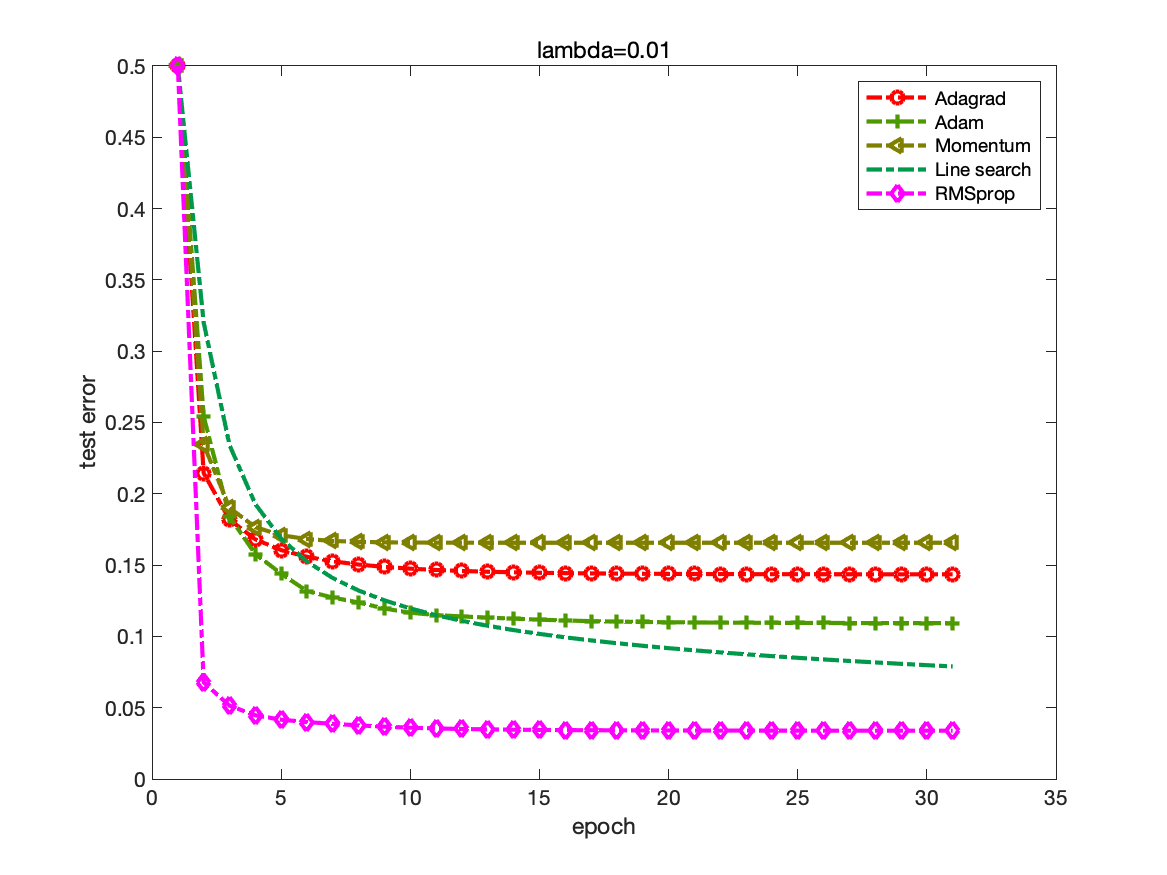
\includegraphics[width=1\linewidth]{./fig/err_g4}
	\caption{Testing error}
\end{minipage}
\caption*{Results on Gisette when $\lambda=0.01$}
\end{figure}
Here in the gradient norm, we omit the $\ell_1$ regularized part since it dominates when $\lambda$ is large. We see all the three algorithms perform well on the datasets, yielding a relatively high quality solution within only a few epochs. A significant influence of regularization term is shown and the three algorithms have different performance in term of different standards. We observe that Adam and RMSprop outperforms the others in both training error and testing error, which is consistent with our intuition that Adam and RMSprop utilize a kind of self-adaptive stepsize on each component for acceleration. No wonder Adam and RMSprop are so widely used in deep learning. Additionally, Adagrad also behaves well. On the other hand, the SGD with linesearch converges faster in primal gradient norm and testing error than the momentum algorithm in the first dataset. This indicates its competitive stability and ability of restoration in the theoretical base of convergence analysis, as well as easy implementation. The faster convergence of the momentum in training error (with regularization term) compared to SGD with linesearch shows the superiority of momentum in preserving the descent direction, since we did not add a momentum term to SGD with linesearch. In this kind of median-size problems, these algorithms show a fast convergence. We leave further discussion of second-order algorithms in the future due to space limitation. Anyway, we have completed all requirements including extra-credits in this assignment.
%\nocite{*}
\bibliographystyle{plain}  
\bibliography{ref}
\end{document}